
% VLDB template version of 2020-08-03 enhances the ACM template, version 1.7.0:
% https://www.acm.org/publications/proceedings-template
% The ACM Latex guide provides further information about the ACM template

\documentclass[sigconf, nonacm, pdfa]{acmart}

%% The following content must be adapted for the final version
% paper-specific
\newcommand\vldbdoi{10.14778/3828612.3828620}
\newcommand\vldbpages{2630 - 2642}
% issue-specific
\newcommand\vldbvolume{19}
\newcommand\vldbissue{10}
\newcommand\vldbyear{2026}
% should be fine as it is
\newcommand\vldbauthors{\authors}
\newcommand\vldbtitle{\shorttitle} 
% leave empty if no availability url should be set
\newcommand\vldbavailabilityurl{https://github.com/nju-websoft/MonoGST}
% whether page numbers should be shown or not, use 'plain' for review versions, 'empty' for camera ready
\newcommand\vldbpagestyle{empty} 
\usepackage[a-2b]{pdfx}
\usepackage{amsfonts}
\usepackage{color}
\usepackage{booktabs}
\usepackage{multirow}
\usepackage{url}
\usepackage{xspace}
\usepackage{listings}

\usepackage{overpic}
\usepackage{subfig}
\usepackage{graphicx}
\usepackage{grffile}
\usepackage{makecell}
\usepackage{setspace}
\usepackage{enumitem}
\usepackage{adjustbox}
\usepackage{hyperref}
\usepackage[normalem]{ulem}

% \newcolumntype{L}[1]{>{\raggedright\arraybackslash}p{#1}}
% \newcolumntype{C}[1]{>{\centering\arraybackslash}p{#1}}
% \newcolumntype{R}[1]{>{\raggedleft\arraybackslash}p{#1}}

\newtheorem{theorem}{Theorem}
\newtheorem{lemma}{Lemma}

\usepackage[ruled,linesnumbered,noend,boxed]{algorithm2e}
\SetKwInOut{KIN}{Input }
\SetKwInOut{KOUT}{Output }
\SetKw{Break}{break}
\SetKw{Continue}{continue}
\SetEndCharOfAlgoLine{\string;}
\SetArgSty{textup}
% \usepackage{algorithmicx}
% \newcommand{\KwTo}{\textbf{to}\ }
% \algnewcommand\algorithmicto{\textbf{to}}
% \algrenewtext{For}[3]{\algorithmicfor\ #1 \gets #2 \algorithmicto\ #3 \algorithmicdo}

\DeclareMathOperator*{\argmin}{arg\,min}
\DeclareMathOperator*{\argmax}{arg\,max}
\newcommand{\len}{\ensuremath{\mathtt{len}}\xspace}
\newcommand{\dist}{\ensuremath{\mathtt{dist}}\xspace}
\newcommand{\getD}{\ensuremath{\mathtt{DistQuery}}\xspace}
\newcommand{\getSP}{\ensuremath{\mathtt{SPQuery}}\xspace}
\newcommand{\w}{\ensuremath{\mathtt{w}}\xspace}
\newcommand{\Basic}{\ensuremath{\mathtt{MonoGST}}\xspace}
\newcommand{\Improved}{\ensuremath{\mathtt{MonoGST+}}\xspace}
\newcommand{\num}{\ensuremath{\mathtt{num}}\xspace}
\newcommand{\SP}{\ensuremath{\mathtt{SP}}\xspace}
\newcommand{\MST}{\ensuremath{\mathtt{MST}}\xspace}
\newcommand{\ud}{\ensuremath{\mathtt{ud}}\xspace}
\newcommand{\F}{\ensuremath{\mathtt{F}}\xspace}
\newcommand{\bestprefix}{\ensuremath{\mathtt{bpre}}\xspace}
\newcommand{\BuildHeap}{\ensuremath{\mathtt{BuildHeap}}\xspace}

% For algorithm name
\newcommand{\BasicPTS}{\ensuremath{\mathtt{MonoGST}}\xspace}
\newcommand{\ImprovPTS}{\ensuremath{\mathtt{MonoGST+}}\xspace}


% For chapter 3
\newcommand{\OptGST}{\ensuremath{\mathtt{OptGST}}\xspace}
\newcommand{\Optstar}{\ensuremath{\mathtt{Optstar}}\xspace}

% For chapter 4
\newcommand{\Pred}{\ensuremath{\mathtt{Pred}}\xspace}
\newcommand{\PartialDijkstra}{\ensuremath{\mathtt{SuspendableDijkstra}}\xspace}
%\newcommand{\PartialDijkstral}{\ensuremath{\mathtt{Suspendable}}\xspace}
%\newcommand{\PartialDijkstrar}{\ensuremath{\mathtt{Dijkstra}}\xspace}

\newcommand{\UpdateCandidate}{\ensuremath{\mathtt{UpdatePrefix}}\xspace}
\newcommand{\ConstructTree}{\ensuremath{\mathtt{ConstructTree}}\xspace}
\newcommand{\DUB}{\ensuremath{\mathtt{DUB}}\xspace}
\newcommand{\Cost}{\ensuremath{\mathtt{Cost}}\xspace}

\newcommand{\new}{\ensuremath{\mathtt{New}}\xspace}
\newcommand{\UpdateUpperBound}{\ensuremath{\mathtt{UpdateBound}}\xspace}
\newcommand{\UpdateUpperBoundfs}{\ensuremath{\mathtt{UpdateUpper}}\xspace}
\newcommand{\UpdateUpperBoundt}{\ensuremath{\mathtt{Bound}}\xspace}

\newcommand{\Pre}{\ensuremath{\texttt{All}}\xspace}
\newcommand{\Sum}{\ensuremath{\texttt{Sum}}\xspace}

% Datesets Name
\newcommand{\Toronto}{\ensuremath{\mathtt{Toronto}}\xspace}
\newcommand{\DBLP}{\ensuremath{\mathtt{DBLP}}\xspace}
\newcommand{\MovieLens}{\ensuremath{\mathtt{MovieLens}}\xspace}

\newcommand{\MONDIAL}{\ensuremath{\mathtt{MONDIAL}}\xspace}
\newcommand{\LinkedMDB}{\ensuremath{\mathtt{LinkedMDB}}\xspace}
\newcommand{\DBpedia}{\ensuremath{\mathtt{DBpedia}}\xspace}

% \newcommand{\beq}[1]{\resizebox{\columnwidth}{!}{$ #1 $}}


\newcommand{\shan}[1]{\textcolor{red}{#1}}
\newcommand{\gong}[1]{\textcolor{green}{#1}}
\newcommand{\dew}[1]{#1}
% \newcommand{\dew}[1]{{\textcolor{blue}{#1}}}

\begin{document}

% ==================== Response to Revision ====================
% \twocolumn[]
% \thispagestyle{plain}

\begin{center}
    {\LARGE\bfseries Authors' Response to Reviews\par}
    \vspace{1em}
\end{center}

\noindent\textbf{Dear Reviewers,}

\noindent We thank you for your careful reading of our manuscript and for your valuable feedback. In response to the meta-review and the reviewers' comments, we have revised the manuscript extensively. Below we provide a point-by-point response to the concerns raised.

\section*{Meta-Reviewer}
The reviewers think that the problem is interesting. However, they also demand \uline{improvements to the content writing and experimentation details}. Please improve according to their comments.

\textbf{Response:} We have carefully revised the manuscript according to the reviewers' comments. In particular, we \textbf{added the requested experiments}. We also polished the manuscript throughout by \textbf{redefining the running example and related explanations}, making the presentation smoother and easier to follow.

\section*{Reviewer \#2}

\textbf{O1:} In the experiments, the values of g are set to $[5, 8]$ which are too small. This setting is not super meaningful to me. To see this, according to Table 1, if $g$ is such a small constant, the running time of ImprovAPP is bounded by $O(m + n^2)$ which is better than the one of \Improved $O(nm + n^2)$. Moreover, in this case, the approximation ratios of both these algorithms are considered $O(1)$. These assertions are also evidenced by the experimental results. In Table 3, the running time of ImprovAPP is faster than \Improved in most of datasets (except for LinkedMDB) and its average NWeight is competitive to that of \Improved, where both of them are very close to 1. Therefore, from these experimental results, the effectiveness of \Improved is less significant. \uline{The authors should conduct experiments on these datasets with large values of $g$.}

\textbf{Response:} Following this request for larger-$g$ experiments, we conducted additional experiments with $g$ ranging from 5 to 50. We added a new \textbf{Robustness Analysis} in \textbf{Section~\ref{subsec: sensitivity}} to evaluate how the algorithms perform as $g$~increases. The new results in \textbf{Figure~\ref{fig: sens_gf} (left)} show that for larger values of~$g$, \ImprovPTS robustly delivers high-quality solutions and outperforms ImprovAPP, and its running time is empirically linear in~$g$.

\textbf{O2:} The dedicated experimental study on impact of the average group sizes $f$ is missing. It is unclear that why $f$ is set to $\{200, 400, 800, 1600\}$. \uline{Experiments on $f$ is needed.} The impact of a large $g$ with small $f$ is unclear from the current experimental results.

\textbf{Response:} Following this request for experiments on~$f$, we conducted additional experiments with $f$ ranging from~200 to~2000. We added a new \textbf{Robustness Analysis} in \textbf{Section~\ref{subsec: sensitivity}} to evaluate how the algorithms perform as $f$~increases. The new results in \textbf{Figure~\ref{fig: sens_gf} (right)} show that for larger values of~$f$, \ImprovPTS robustly delivers high-quality solutions and outperforms ImprovAPP, and its running time is empirically linear in~$f$.

\textbf{O3:} As mentioned in O1, the practical performance of \Improved seems not substantially better than the existing SOTA ImprovAPP. \uline{The authors need to design experiments to show the superiority of their algorithm.}

\textbf{Response:} Following this request for experiments that demonstrate the superiority of \ImprovPTS over ImprovAPP, we strengthened the evaluation from both the worst-case quality and the quality in varying settings. In \textbf{Section~\ref{subsubsec: main-exper-results}}, the \textbf{Effectiveness Results (NWeight)}, the maximum NWeight reached by ImprovAPP is consistently larger than that of \ImprovPTS, with their gap more pronounced on larger graphs, up to $40\%$ on DBpedia; this is followed by a \textbf{case study} related to \textbf{Figure~\ref{fig:TF}}. We added a new \textbf{Scalability Analysis} in \textbf{Section~\ref{subsec: scalability}}, where on almost all graphs, \Improved outputs better results than ImprovAPP; we also added a new \textbf{Robustness Analysis} in \textbf{Section~\ref{subsec: sensitivity}}, where the mean weight ratio of ImprovAPP to \ImprovPTS is kept between~1.108 and~1.146. All these results demonstrate the superiority of \ImprovPTS over ImprovAPP.

\section*{Reviewer \#4}

\textbf{D1:} While the holistic analysis is a significant contribution, the current proof for the $O(\sqrt{g})$ approximation ratio is presented in an overly dense manner, making the high-level intuition behind the removal of the logarithmic factor difficult to grasp. \uline{The authors should provide a more intuitive conceptual summary or a high-level roadmap of the proof} to help readers clearly follow the logic of how the 2-star greedy process tightens the standard bound.

\textbf{Response:} Following this request for a clearer proof roadmap, we added a high-level explanation in \textbf{Section~\ref{subsubsec: Appr_prove}}. The added paragraph explains why the well-known bound $O(\sqrt{g}\ln g)$ is loose and highlights the key idea of our tighter analysis, namely to charge each iteration recursively with a decreased number of uncovered groups (i.e.,~$i$ in the following analysis).

\textbf{D2:} While the authors state that existing methods do not scale to large graphs and claim that \Improved scales linearly with graph size, they provide no direct experimental evidence to support this claim. Thus, \uline{the authors are suggested to conduct a scalability study varying the number of vertices and comparing \Improved with selected existing methods}.

\textbf{Response:} Following this request for scalability experiments, we added a new \textbf{Scalability Analysis} in \textbf{Section~\ref{subsec: scalability}} based on a family of subgraphs with increasing numbers of vertices. The new results \textbf{in Figure~\ref{fig: subgraph} (top left)} show that the running time of \Improved increases slowly with~$n$, while several other algorithms show scalability limitations and their curves terminate early.

\textbf{D3:} Although the authors vary the number of groups ($g$) and the average group size ($f$), Table 3 presents only aggregate results, failing to show how these parameters affect algorithm performance independently. \uline{The authors should include detailed sensitivity analyses, such as plots of runtime and NWeight against varying $g$ and $f$}, to demonstrate the algorithm's robustness across different query configurations.

\textbf{Response:} Following this request for sensitivity analyses of $g$ and $f$, we added a new \textbf{Robustness Analysis} in \textbf{Section~\ref{subsec: sensitivity}}. \textbf{Figure~\ref{fig: sens_gf}} plots the distributions of running time and NWeight of \ImprovPTS over all GSTP instances in each setting of~$g$ or~$f$, demonstrating its robustness across different query configurations.

\textbf{D4:} While the paper focuses on execution time, it omits experimental results regarding memory consumption. Given that scalability to large graphs is a core claim, \uline{the authors should provide a comparative analysis of memory usage} to demonstrate the resource efficiency of \Improved relative to other index-free and index-based methods.

\textbf{Response:} Following this request for memory-consumption experiments, we added comparative results of memory use in the \textbf{Scalability Analysis} in \textbf{Section~\ref{subsec: scalability}}. The new results in \textbf{Figure~\ref{fig: subgraph} (top right)} show that \ImprovPTS has the lowest memory use and its space increases slowly with~$n$.

\textbf{D5:} The descriptions of the suspendable Dijkstra search and monotonicity-aware pruning could be supplemented with figures to facilitate a more intuitive understanding of these core technical contributions. \uline{The authors are encouraged to include illustrative examples of these processes} to visualize how the dynamic bounding mechanism and the search space reduction function operate in practice.

\textbf{Response:} Following this request for illustrative examples of the suspendable Dijkstra search and monotonicity-aware pruning, we strengthened our running example. For the suspendable Dijkstra search, we annotated \textbf{Figure~\ref{fig: TF}} with the vertices visited in different calls of \PartialDijkstra and illustrated the dynamic bounding mechanism in the \textbf{Running Example} in \textbf{Section \ref{subsec: sec_dub}}. For monotonicity-aware pruning, we added a \textbf{Running Example} in \textbf{Section~\ref{subsec: mono_upt}} to illustrate how the prefix extends over iterations.

\section*{Reviewer \#5}

\textbf{R1:} \uline{The revision should analyze how performance changes with the number of groups ($g$), quantify the benefit of early termination in suspendable Dijkstra (e.g., visited nodes/work saved versus full SSSP), and evaluate the effect of prefix pruning.}

\textbf{Response:} Following this request to analyze the effects of $g$, suspendable Dijkstra, and prefix pruning, we extended our experiments in three aspects.
First, we added a dedicated \textbf{Robustness Analysis} in \textbf{Section~\ref{subsec: sensitivity}}. The results in \textbf{Figure~\ref{fig: sens_gf} (left)} show that as $g$~increases, \ImprovPTS robustly delivers high-quality solutions and outperforms ImprovAPP, and its running time is empirically linear in~$g$.
Second, in the \textbf{Efficiency Results (Running Time)} in \textbf{Section~\ref{subsubsec: abl_result}}, we quantified the benefit of early termination by reporting that on different datasets, only an average of 0.02\%--20\% of all vertices are visited when Dijkstra's algorithm is terminated.
Third, also in that section, we added an evaluation of the effect of prefix pruning, reporting an increase in speedup from~21\% to~42\% as $g$~increases from~5 to~8.

\textbf{R2:} \uline{The paper should include an analysis of how choosing the root from the smallest group affects runtime and solution quality}, especially when group sizes are imbalanced.

\textbf{Response:} Following this request for root-selection analysis, we added an ablation study to compare three root-selection strategies in \textbf{Section~\ref{subsec: able}}: the default smallest-group strategy, compared with the median group and the largest group. The new results in \textbf{Table~\ref{table: abl}} show that switching from the smallest group to the median or largest group leads to consistent increases in running time, while it has little effect on solution quality, demonstrating the cost-effectiveness of the smallest-group strategy.

\textbf{R3:} \uline{The revision should add a small but concrete example explaining the 2-star construction and the main optimization ideas} (e.g., suspendable Dijkstra/prefix pruning/path re-selection).

\textbf{Response:} Following this request for a concrete example of our approach, we strengthened our running example. We revised \textbf{Figure~\ref{fig: TF}} and revised the \textbf{Running Example} in \textbf{Section~\ref{subsec: basic_design}} and \textbf{Section~\ref{subsec: improved-design}} to illustrate the 2-star construction, added a concrete \textbf{Running Example} in \textbf{Section~\ref{subsec: sec_dub}} for suspendable Dijkstra, and added a \textbf{Running Example} in \textbf{Section~\ref{subsec: mono_upt}} for prefix pruning. The effect of path re-selection is illustrated by different trees shown in \textbf{Figure~\ref{fig: TF}}, and this case study is included at the end of the \textbf{Efficiency Results (Running Time)} in \textbf{Section~\ref{subsubsec: main-exper-results}}.

\textbf{R4:} \uline{The paper should include at least one small-graph visualization or case study comparing the trees returned by \Improved, \Basic, and one representative baseline.}

\textbf{Response:} Following this request for a small-graph visualization and case study, we extended \textbf{Figure~\ref{fig: TF}}, which now compares the trees returned by ImprovAPP, \Basic, and \Improved. We also added a corresponding case study at the end of the \textbf{Efficiency Results (Running Time)} in \textbf{Section~\ref{subsubsec: main-exper-results}}.

\textbf{R5:} In particular, \uline{the authors should clarify how timeout cases are handled in quality comparisons, and report whether the conclusions change under an evaluation that includes all instances} (for example, by treating timeout cases conservatively). In addition, if polylogarithmic-approximation methods are too expensive for the full datasets, they should be evaluated on smaller graphs/subgraphs or otherwise \uline{discussed more explicitly to better position the proposed method}.

\textbf{Response:} Following this request to clarify the handling of timeouts, we revised the description of the evaluation metrics in \textbf{Section~\ref{subsubsec: eva-metrics}} to explain how timeout cases are handled in quality comparisons. We also added a \textbf{Scalability Analysis} in \textbf{Section~\ref{subsec: scalability}}, where all baselines are practical on the smallest subgraph and can be compared directly. The new results in \textbf{Figure~\ref{fig: subgraph}} show how the more expensive methods fail as the graph expands, contextualizing quality comparisons in the presence of timeouts. We further clarified about polylogarithmic-approximation methods in \textbf{Section~\ref{subsec: sub-alg}}, explaining that as noted in their papers, they incur large hidden constants and accumulated polylogarithmic factors, hard to perform efficiently in practice (and even hard to implement); they are more oriented towards theoretical analysis than practical deployment.

\textbf{R6:} Since GSTP-style workloads may arise in multi-query scenarios, \uline{the revision should discuss whether any intermediate computation or data structure (e.g., SSSP-related results or ($D^{\mathtt{Sum}})$) can be reused across queries, and what the expected trade-offs would be.} A brief empirical study would be ideal, but at minimum the paper should clarify this limitation and the potential for reuse.

\textbf{Response:} Following this request to discuss reuse across queries, we added a brief discussion in \textbf{Section~\ref{subsubsec: basic-time}}, explaining that in multi-query scenarios, intermediate results such as shortest-path trees computed by SSSP can be cached and reused to reduce the time cost of subsequent queries.

\textbf{R7:} \uline{Address minor presentation issues and typos.} The noted wording/grammar issues should be corrected in the revision.

\textbf{Response:} Following this request to address presentation issues and typos, we revised the manuscript to correct all the noted wording and grammar issues, including but not limited to the punctuation in \textbf{Section~\ref{sec: introduction}} and the phrasing in \textbf{Section~\ref{subsec: line-alg}}.
% \clearpage
% \setcounter{page}{1}
% ==================== Response to Revision ====================

\title{A Practical Sublinear Approximation for Group Steiner Tree}

%%
%% The "author" command and its associated commands are used to define the authors and their affiliations.
\author{Yuxuan Yang}
\affiliation{%
  \institution{Nanjing University}
  \department{State Key Laboratory of Novel Software Technology}
  \city{Nanjing}
  \state{Jiangsu}
  \country{China}
}
\email{yxyang@smail.nju.edu.cn}

\author{Sirui Chen}
\affiliation{%
  \institution{Nanjing University}
  \department{State Key Laboratory of Novel Software Technology}
  \city{Nanjing}
  \state{Jiangsu}
  \country{China}
}
\email{siruichen@smail.nju.edu.cn}

\author{Zhuolin He}
\affiliation{%
  \institution{Nanjing University}
  \department{State Key Laboratory of Novel Software Technology}
  \city{Nanjing}
  \state{Jiangsu}
  \country{China}
}
\email{zhuolin.he@smail.nju.edu.cn}

\author{Gong Cheng}
\authornote{Corresponding author.}
\affiliation{%
  \institution{Nanjing University}
  \department{State Key Laboratory of Novel Software Technology}
  \city{Nanjing}
  \state{Jiangsu}
  \country{China}
}
\email{gcheng@nju.edu.cn}

%%
%% The abstract is a short summary of the work to be presented in the
%% article.
\begin{abstract}
The Group Steiner Tree Problem (GSTP) is widely used in graph data management and mining, yet existing algorithms trade off practical efficiency against approximation quality: efficient methods offer only linear guarantees, while those with sublinear guarantees fail to scale to large graphs. In this paper, we present \Improved, a novel algorithm for GSTP that breaks this trade‑off by achieving a sublinear approximation while matching the running time of state‑of‑the‑art linear‑approximation solvers. Our approach extends a 2‑star‑based reduction to weighted set cover with a suspendable search and a monotonicity‑ and unimodality‑aware pruning strategy to eliminate redundant computation. Experiments on multiple real‑world datasets demonstrate the effectiveness and efficiency of \Improved, providing a practical, high‑quality solution for GSTP applications.
\end{abstract}

\maketitle

%%% do not modify the following VLDB block %%
%%% VLDB block start %%%
\pagestyle{\vldbpagestyle}
\begingroup\small\noindent\raggedright\textbf{PVLDB Reference Format:}\\
\vldbauthors. \vldbtitle. PVLDB, \vldbvolume(\vldbissue): \vldbpages, \vldbyear.\\
\href{https://doi.org/\vldbdoi}{doi:\vldbdoi}
\endgroup
\begingroup
\renewcommand\thefootnote{}\footnote{\noindent
This work is licensed under the Creative Commons BY-NC-ND 4.0 International License. Visit \url{https://creativecommons.org/licenses/by-nc-nd/4.0/} to view a copy of this license. For any use beyond those covered by this license, obtain permission by emailing \href{mailto:info@vldb.org}{info@vldb.org}. Copyright is held by the owner/author(s). Publication rights licensed to the VLDB Endowment. \\
\raggedright Proceedings of the VLDB Endowment, Vol. \vldbvolume, No. \vldbissue\ %
ISSN 2150-8097. \\
\href{https://doi.org/\vldbdoi}{doi:\vldbdoi} \\
}\addtocounter{footnote}{-1}\endgroup
%%% VLDB block end %%%

%%% do not modify the following VLDB block %%
%%% VLDB block start %%%
\ifdefempty{\vldbavailabilityurl}{}{
\vspace{.3cm}
\begingroup\small\noindent\raggedright\textbf{PVLDB Artifact Availability:}\\
The source code, data, and/or other artifacts have been made available at \url{\vldbavailabilityurl}.
\endgroup
}
%%% VLDB block end %%%

\section{Introduction}
\label{sec: introduction}
The Group Steiner Tree Problem (GSTP) is a classical NP-hard optimization problem. Given a graph with $n$ vertices, $m$ weighted edges, and a query consisting of $g$ groups---each group is a subset of vertices, the goal is to find a tree that contains at least one vertex from each group while minimizing the total edge weight.

% Respond Reviewer #4 R5:The descriptions of the suspendable Dijkstra search and monotonicity-aware pruning could be supplemented with figures to facilitate a more intuitive understanding of these core technical contributions. The authors are encouraged to include illustrative examples of these processes to visualize how the dynamic bounding mechanism and the search space reduction function operate in practice.

% Respond Reviewer #5 R3: The revision should add a small but concrete example explaining the 2-star construction and the main optimization ideas (e.g., suspendable Dijkstra/prefix pruning/path re-selection).
% Respond Reviewer #5 R4: The paper should include at least one small-graph visualization or case study comparing the trees returned by MonoGST+, MonoGST, and one representative baseline.
\begin{figure*}[t]
  \centering
  % ===== Row 1: TF (left) and KS (right) =====
  \begin{minipage}[t]{0.347\textwidth}
    \centering
    \subfloat[\dew{The top part is a social network of experts $\{1,2,\dots,13\}$; each vertex is annotated with the corresponding expert’s skill set, and edge weights measure relationship weakness. Each skill induces a group of experts, e.g., $s_1\mapsto\{1\}$ and $s_2\mapsto\{5,6,9\}$. Given a set of required skills as a query $Q=\{s_1,\dots,s_8\}$, the three GSTs in the bottom part represent feasible teams with weights $24$, $22$, and $20$ computed by ImprovAPP, \Basic, and \Improved, respectively.} \label{fig: TF}]{%
      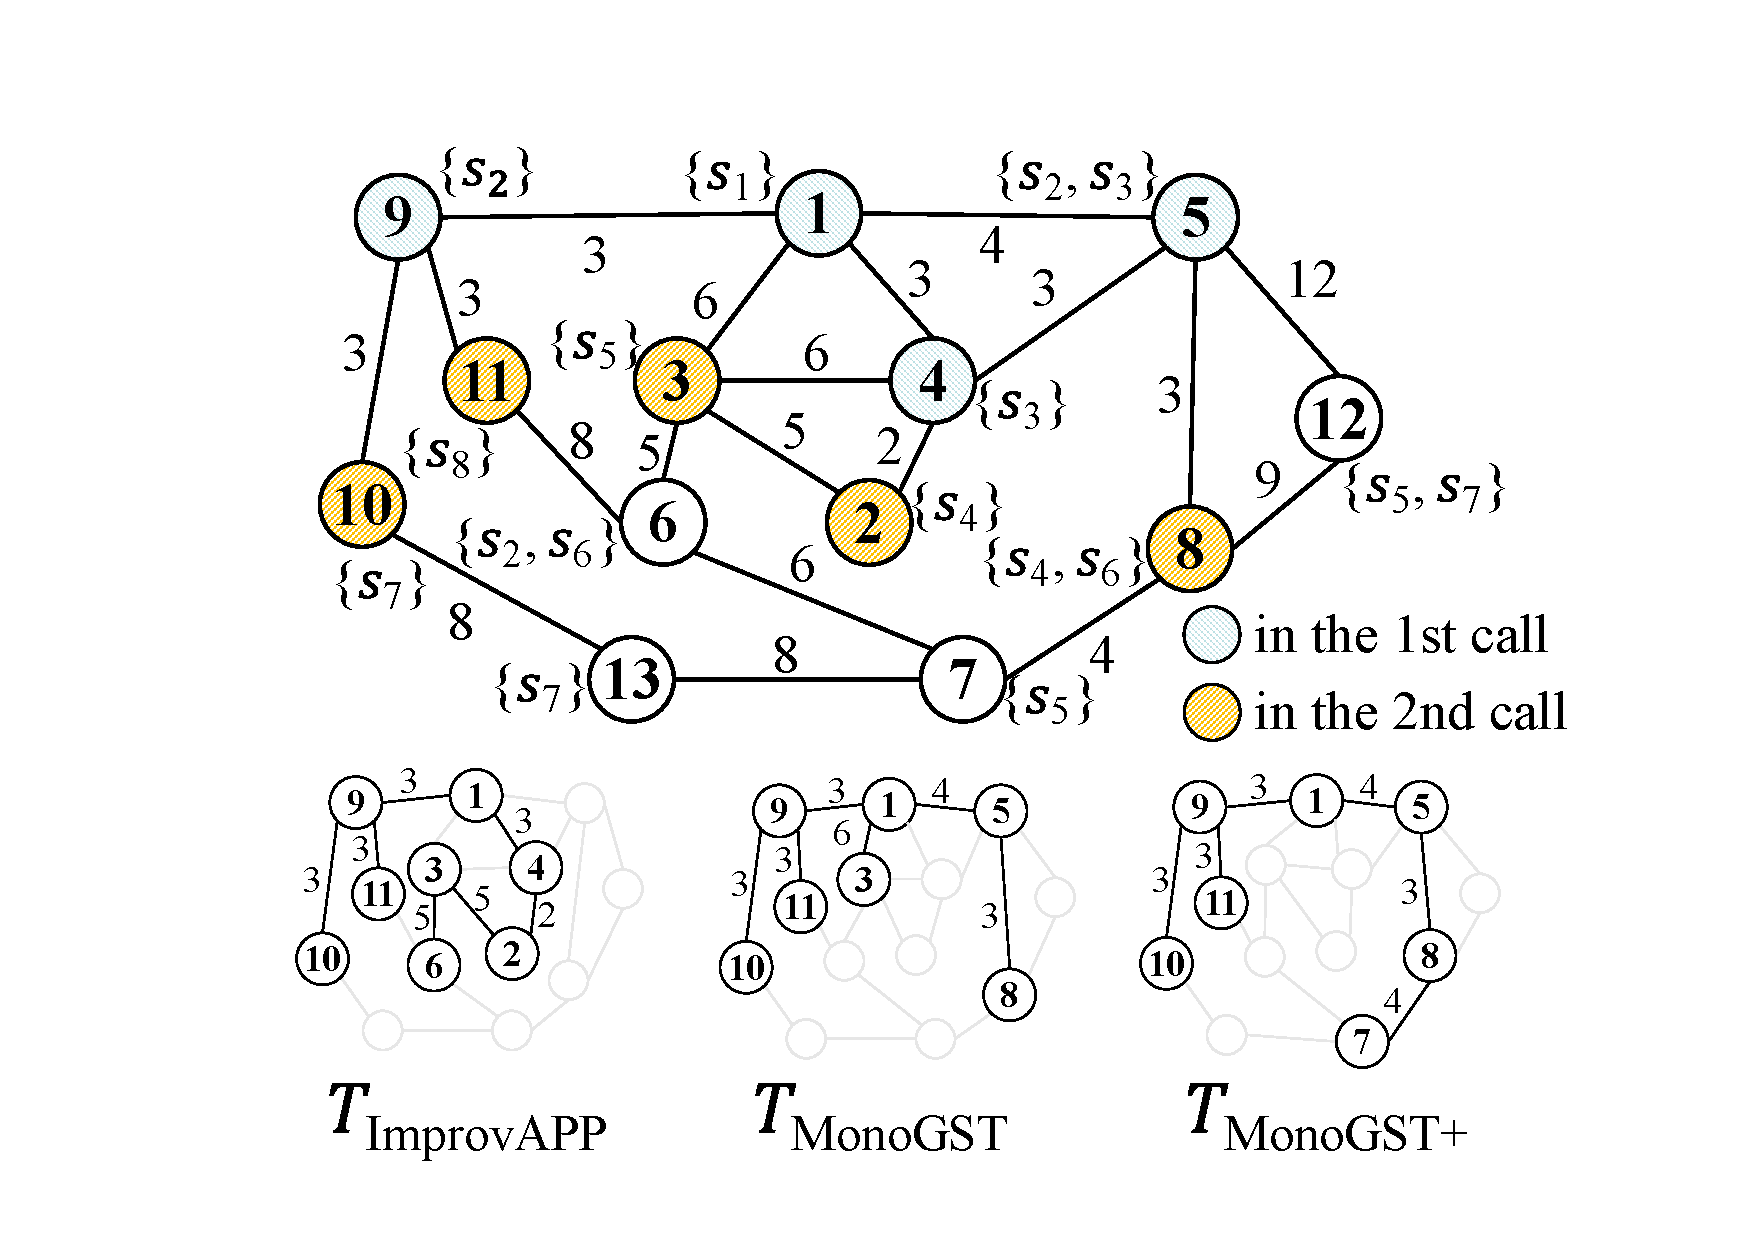
\includegraphics[width=\linewidth]{fig/application/ill7.pdf}%
      \label{fig:TF}%
    }
  \end{minipage}\hfill
  \begin{minipage}[t]{0.32\textwidth}
    \centering
    \subfloat[Consider a technology-themed KG, along with an illustrative query ``Apple Innovation Expo California.'' For this query, each keyword is mapped to a group of entity vertices in the KG: $\textit{Apple}\mapsto \{\#1,\#2\}$, $\textit{Innovation}\mapsto \{\#7,\#8\}$, $\textit{Expo}\mapsto \{\#7,\#10\}$, and $\textit{California}\mapsto \{\#4,\#11\}$. The dashed-boxed subgraph~$T$ is a feasible answer to this query; this GST simultaneously covers and connects all the four keyword-induced groups. \label{fig: KS}]{%
      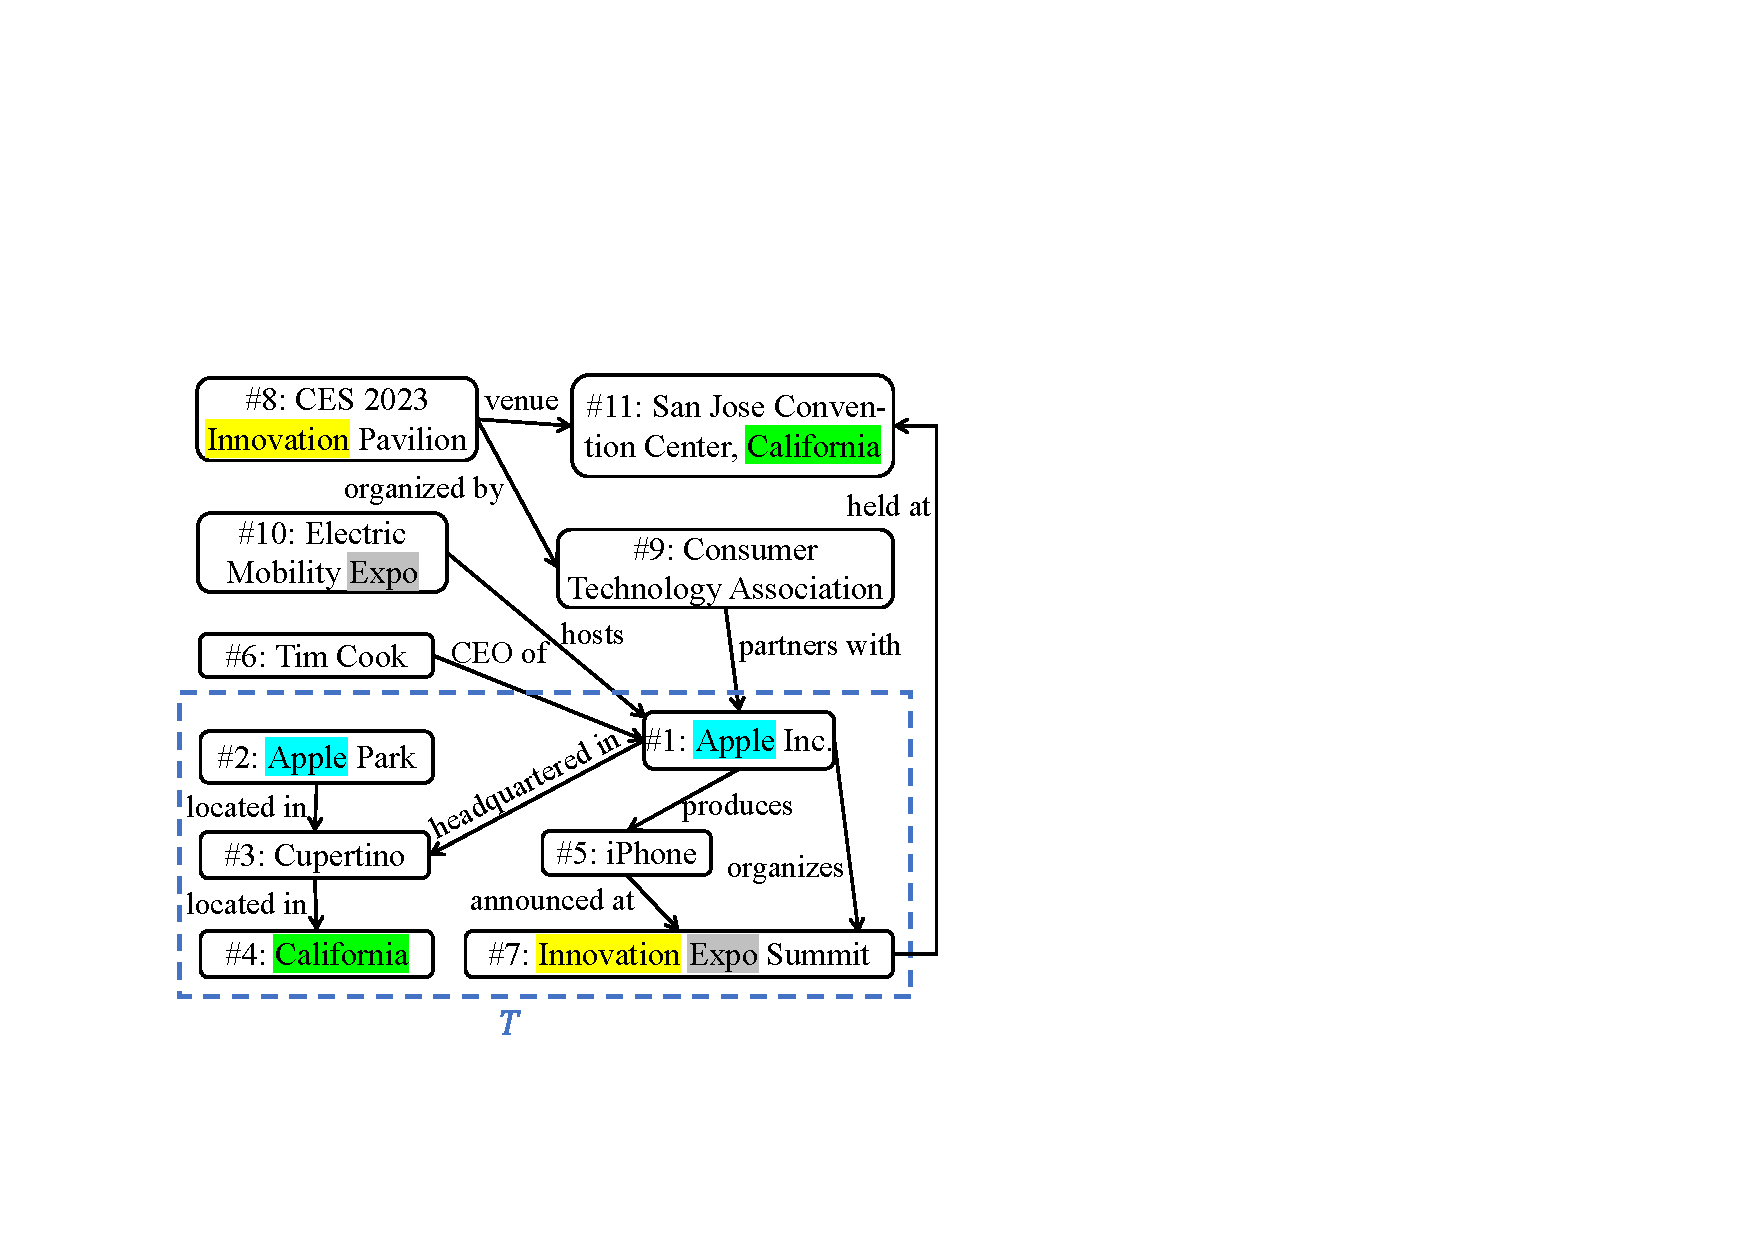
\includegraphics[width=\linewidth]{fig/application/pic2b.pdf}%
      \label{fig:KS}%
    }
  \end{minipage}
  \hfill
  \begin{minipage}[t]{0.314\textwidth}
    \centering
    \subfloat[The top part is a KG; vertices (or edges) with the same color have the same EDP (or LP) and form a group. Subdividing the colored edges by inserting vertices and removing classes (dotted boxes) and literals (quoted) yields an ELG in the bottom part. The dashed-boxed GST~$T$ covers all pattern-induced groups. Extending it back to a subgraph of the original KG by restoring the removed classes and literals, we will obtain a feasible pattern-coverage summary. \label{fig: KGS}]{%
      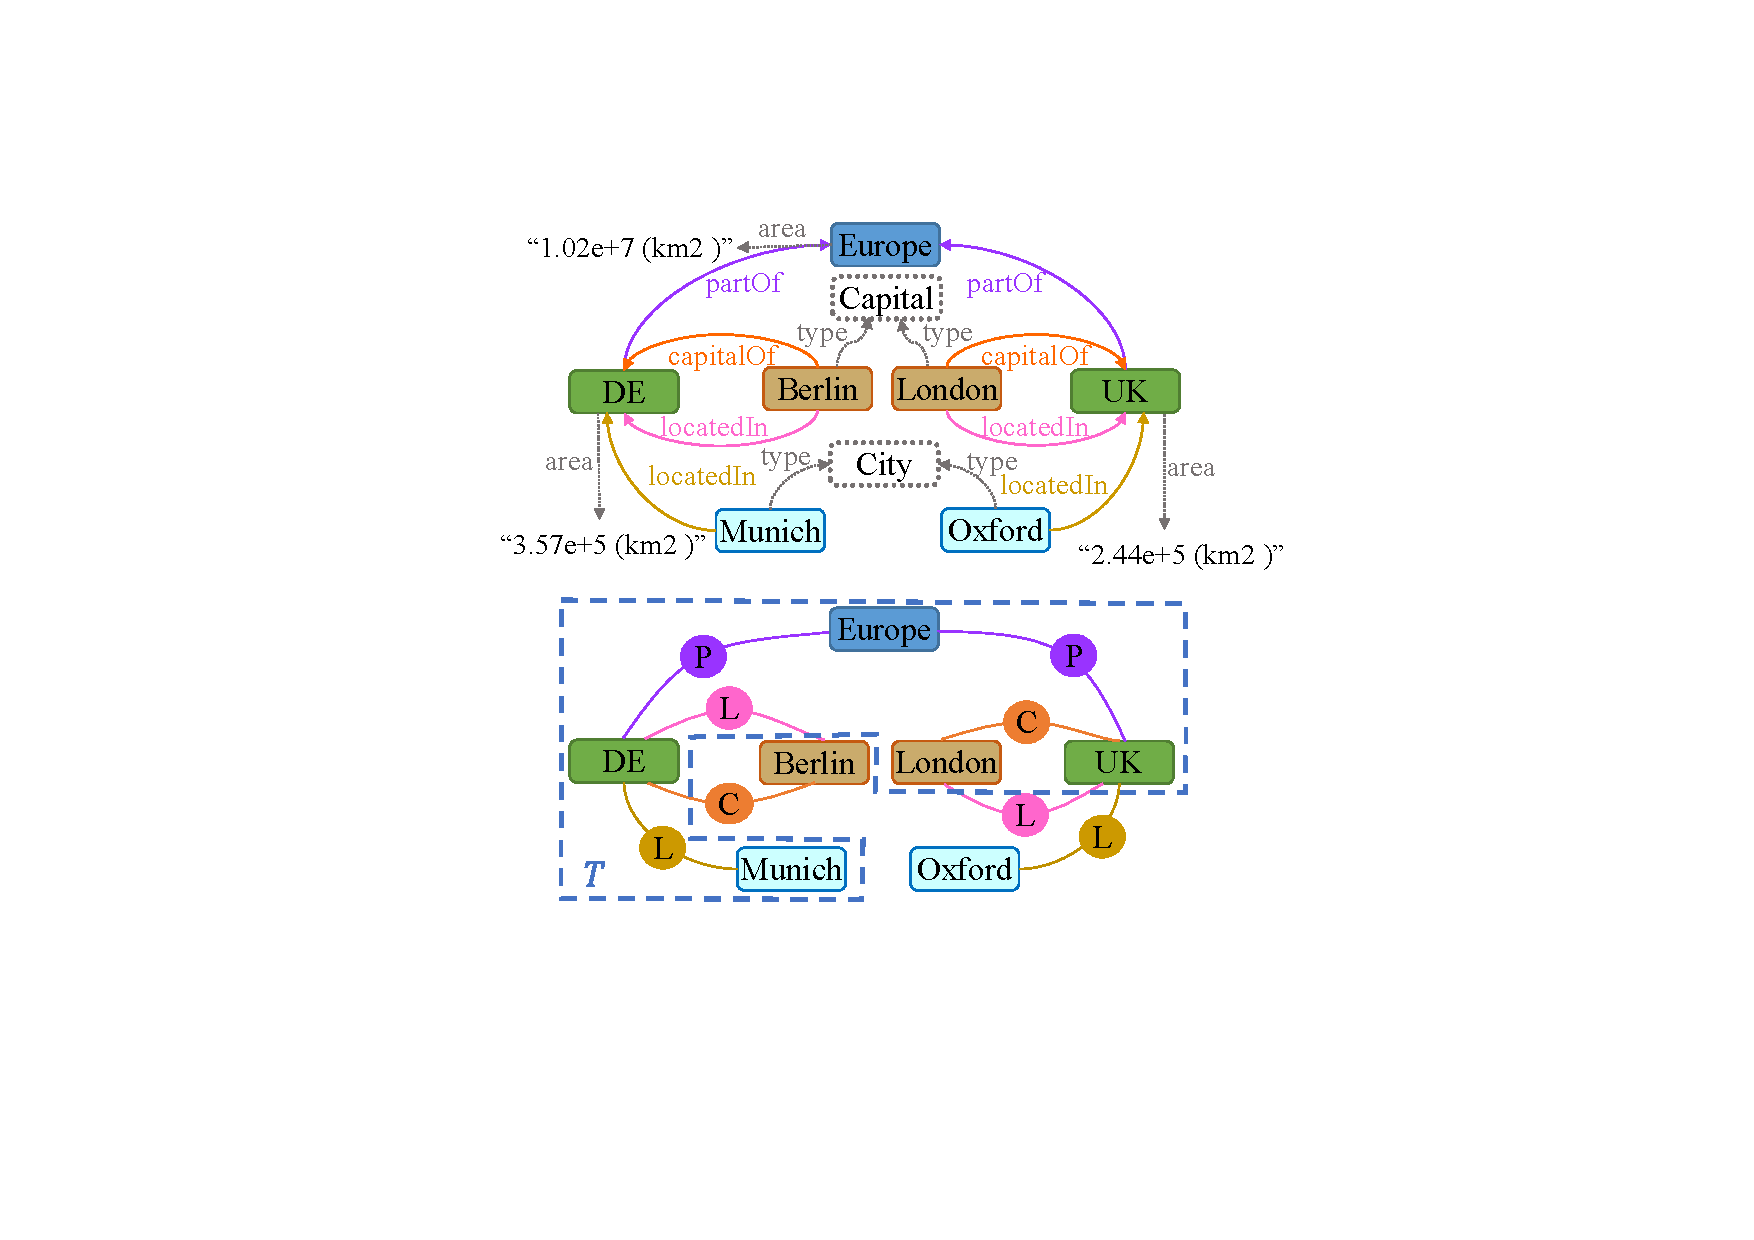
\includegraphics[width=\linewidth]{fig/application/pic3c.pdf}%
      \label{fig:KGS}%
    }
  \end{minipage}

  % \vspace{1ex}

  % % ===== Row 2: three columns (KGS_1 | (KGS_2 over KGS_3) | KGS_4) =====
  % \begin{minipage}[t]{0.372\textwidth}
  %   \centering
  %   \subfloat[An example of RDF Dataset, vertices or edges with the same color indicate that they belong to the same type. \label{fig: KGS_1}]{%
  %     \includegraphics[width=\linewidth]{fig/application/KGS1_.pdf}%
  %     \label{fig:KGS1}%
  %   }
  % \end{minipage}\hfill
  % \begin{minipage}[t]{0.27\textwidth}
  %   \centering
  %   \subfloat[The Entity-Link Graph (ELG) converted from RDF and a feasible GST covering all types in the ELG. \label{fig: KGS_23}]{%
  %     \includegraphics[width=\linewidth]{fig/application/KGS23.pdf}%
  %     \label{fig:KGS1}%
  %   }
  % \end{minipage}\hfill
  % \begin{minipage}[t]{0.34\textwidth}
  %   \centering
  %   \subfloat[Extend the GST to obtain the Pattern-Coverage Snippet. \label{fig: KGS_4}]{%
  %     \includegraphics[width=\linewidth]{fig/application/KGS4.pdf}%
  %     \label{fig:KGS4}%
  %   }
  % \end{minipage}

  \caption{Application scenarios of GSTP.}
  \label{fig: application}
\end{figure*}

% Convert each RDF edge into a vertex and remove gray types and literals to obtain an Entity-Link Graph (ELG). Next, in the ELG, find a minimum subgraph that covers all types; each type corresponds to a set of vertices, so this can be solved via GST. The figure above shows the ELG corresponding to Fig.~\ref{fig: KGS_a} and a valid subgraph of this ELG that covers all types.

\textbf{Application Scenarios.}
GSTP finds applications in the following representative scenarios in graph data management and mining.

\textit{Team Formation.} In social networks,
\iffalse~\cite{TF_3}\fi
vertices represent experts annotated with skills, edges encode acquaintance or collaboration, and smaller edge weights indicate closer relationships. Expert team formation~\cite{TF_4, TF_5} requires the selection of a team of experts whose collective skills cover a specified set while maintaining strong connectivity. In GSTP-based solutions~\cite{TF_3\iffalse TF_1\fi, ImprovAPP}, each required skill corresponds to a group of experts who possess that skill, and a small-weight GST corresponds to a cohesive team. See Figure~\ref{fig: TF}.

\textit{Keyword-Based Exploration.} In knowledge graphs (KGs)~\cite{KG_D}, entities are vertices, and relations are edges; relational databases are converted into graphs where tuples are vertices and foreign keys are edges, often weighted. Keyword-based exploration~\cite{KS_3,\iffalse KS_2\fi KS_1} helps users extract relevant structures. GSTP-based solutions~\cite{KS_6, KS_7\iffalse KS_4\fi, KS_5} map each input keyword to a group of matching vertices and return a minimum-weight tree covering all groups. See Figure~\ref{fig: KS}.

\textit{Knowledge Graph Summarization.} To reuse a KG, its summary~\cite{KS_3, KGS_3} provides users with an overview of its core content. The state-of-the-art Pattern-Coverage Snippet Generation (PCSG) method~\cite{KGS_1} builds an Entity-Link Graph (ELG) from a KG and uses Entity Description Pattern (EDP) and Link Pattern (LP) to classify entities and relations into groups, respectively. This GSTP-based solution induces an optimal summary with the greatest compression from a smallest subgraph of the ELG showing all patterns. See Figure~\ref{fig: KGS}.

\textit{Very-Large-Scale Integration.} In integrated circuit design, min-cost routing~\cite{VLSI_3} connects multiple equivalent pins. GSTP-based solutions~\cite{VLSI_1, VLSI_2} run on the Hanan grid reduction of a circuit net.

% \textit{Pathway Discovery in Metabolic Networks.} In computational biology, identifying metabolic pathways can be modeled as GSTP~\cite{PI}, illustrating an interdisciplinary application.

\textbf{Motivation.} GSTP is NP-hard~\cite{ProveNP}. Exact algorithms such as DPBF~\cite{KS_5} and PrunedDP++~\cite{PrunedDP} have an exponential running time in the number of groups~$g$ and are difficult to scale to large graphs. This motivates \emph{practical approximation algorithms}. The state of the art includes ImprovAPP~\cite{ImprovAPP} and the index-based KeyKG$^+$~\cite{KeyKG}.
% using a distance oracle~\cite{HL_INTRO} for shortest-path queries and requiring substantial preprocessing time.
They guarantee a $(g-1)$ approximation, i.e., an approximation ratio linear in~$g$. Earlier algorithms such as BANKS~\cite{BANKS}, BANKS-II~\cite{BANKS2}, and BLINKS~\cite{BLINKS} also provide $O(g)$-approximation guarantees.
% but tend to be less efficient on large graphs~\cite{KeyKG}.
All these approaches are inspired by the so-called 1-star structure~\cite{gsub1_source}.

For a \emph{more accurate approximation}, PartialOPT~\cite{ImprovAPP} achieves a $(g-h+1)$ approximation with a parameter $h$, but its running time grows exponentially with~$h$. There are also algorithms with polylogarithmic approximation ratios~\cite{PolyAppr_1, PolyAppr_2}, embedding the graph into a tree metric to solve. However, they are primarily of theoretical interest.
% and become inefficient for large graphs, e.g.,~relying on linear programming (LP) solvers.
Besides, while using the $d$-star structure has the potential to produce a ratio sublinear in~$g$, experimental validation is lacking for large graphs, e.g.,~the 2-star heuristic~\cite{dstar1,dstar2} requiring expensive all-pairs shortest path computation, and the reduction to the Directed Steiner Tree Problem (DSTP)~\cite{D_STP}.

\emph{In summary, existing practical methods typically have mediocre (\dew{i.e.,}~linear) approximation guarantees, while methods with stronger (\dew{i.e.,}~sublinear) guarantees still lack scalability validation.} Table~\ref{table: Algorithms Comparison} summarizes their time complexities and approximation ratios.

\textbf{Our Work.}
To bridge this performance trade-off, our goal is to develop a practical GST algorithm that is \emph{both effective}, providing a sublinear approximation guarantee, \emph{and efficient}, with a speed on par with the fastest index-free linear-approximation algorithms.

% Section~\ref{sec: preliminaries} formulates GSTP and reviews the 2-star structure. Section~\ref{sec: basic}
Specifically, we first propose a basic two-step algorithm \BasicPTS, which greedily approximates via 2-star based on distances calculated by Dijkstra's algorithm and non-trivially achieves an approximation ratio $O(\sqrt g)$.
% In Section~\ref{sec: improved},
Our improved algorithm \ImprovPTS incorporates a \emph{suspendable Dijkstra's algorithm} to calculate distances as needed, leverages the \emph{monotonicity and unimodality of the greedy function} to prune the search space, and constructs a GST from a 2-star through \emph{a greedy re-selection of paths} to enhance the approximation.
% Section~\ref{sec: experiments} empirically demonstrates the efficiency and effectiveness of our approach in multiple scenarios. Finally, Section~\ref{sec: relatedwork} discusses related work and Section~\ref{sec: conclusion} concludes the paper.
Our technical contributions are as follows.
\begin{itemize}
  \item For \BasicPTS, which greedily solves a weighted set cover problem to approximate an optimum 2-star and converts it into a GST, we perform a holistic analysis of this two-step approximation, producing a guaranteed ratio of $O(\sqrt g)$.
  \item In \ImprovPTS, we embed the set cover procedure within Dijkstra's algorithm to establish a dynamic bounding mechanism and exploit the monotonicity and unimodality of the greedy function, substantially pruning the search space.
\end{itemize}
% \textbf{Motivation.} Because the problem is NP-Hard, research on efficient algorithms focuses on approximation algorithms. In the past, Most of the work can not take into account both the practical operation and theoretical approximation ratio. For example, in recent years, algorithms such as KeyKG ~\cite{DBLP:conf/www/Shi0K20} using index and ImprovAPP and PartialOPT ~\cite{DBLP:journals/pvldb/SunX0HL021} without index have an approximate ratio of around $g-1$.

% However, some algorithms with good theoretical approximation, their actual running speed will be unsatisfactory. For example, 2-star ~\cite{DBLP:conf/date/HelvigRZ98,DBLP:conf/ispd/BatemanHRZ97} algorithm does not have enough space to index $O(1)$ time-cost queries on large graphs, and its own running speed is very complex with respect to $n$ and $g$, and the actual running speed is also very slow. Other algorithms based on linear programming and rounding, such as polylogarithmic-approximation algorithm ~\cite{DBLP:journals/jal/GargKR00}, but are also obviously not feasible to run on actual large graphs. 

% Therefore, an algorithm that has a lower approximation ratio of linear theory about g and can run on real graphs is needed.

% \textbf{Our work.} In this paper, we propose new efficient sublinear approximation ratio algorithms based on 2-star method, which also has $O(\sqrt{g}\ln{g})$ approximation ratio. We reexamine the problem from the perspective of set coverage, and give new weight functions and property derivations. Based on the weight function, we carry out a series of pruning, which greatly improves the actual operation efficiency of the algorithm. \shan{TODO}

\begin{table}[t]
    \centering
    \caption{Comparison between GST algorithms.}
    \label{table: Algorithms Comparison}
    \resizebox{\linewidth}{!}{
    \begin{tabular}{lrr}
        \toprule
        Algorithm & Time Complexity & Approx. Ratio \\
        \midrule
%        \multicolumn{3}{l}{\emph{Exact algorithms:}}\\
%        DPH & $O(3^g*n^2+2^gnm)$ & $1$\\
        DPBF & $O(3^gn+2^g((g+\log{n})n+m))$ & $1$\\
        PrunedDP$++$ & $O(3^gn+2^g((g+\log{n})n+m))$ & $1$\\
        \hline
%        \multicolumn{3}{l}{\emph{Sublinear-approximation algorithms:}}\\
        Reduction to tree metric & polynomial & $O(\log ^3n\log g)$\\
        % \gong{Modified-GS} & dependent on LP solvers & $O(\log ^3n\log g)$ \\
        \Basic (ours) & $O(n(m+ng^2+n\log n))$ & $O(\sqrt g)$\\
        \ImprovPTS (ours) & $O(n(m+(n+g)g+n\log n))$ & $O(\sqrt g)$\\
         Reduction to DSTP  & $O(n(mg+ng\log n))$ & $O(\sqrt g)$ \\
         2-star heuristic & $O(n^3+n^2g^2)$ & $O(\sqrt g\ln g)$\\ 
        \hline
%        \multicolumn{3}{l}{\emph{Linear-approximation algorithms:}}\\
        PartialOPT & $O(n(gn+3^hn+2^h(m+hn+n\log{n})))$ & $g-h+1$\\
        KeyKG$^+$ & $O(n^2g+ng^3)$ & $g-1$\\
        ImprovAPP & $O(g(m+n\log{n}+n^2+n\log{g}))$ & $g-1$ \\
        BANKS & $O(n^2\log{n}+nm)$ & $O(g)$\\
        BANKS-II & $O(n^2\log{n}+nm)$ & $O(g)$\\
        BLINKS & dependent on partition & $O(g)$\\
        \bottomrule
    \end{tabular}
    }
\end{table}

Experiments on five diverse real-world datasets demonstrate that \ImprovPTS attains better solution quality than existing approximation algorithms while running as fast as the state-of-the-art index-free linear-approximation solver, thereby bridging the long-standing effectiveness-efficiency trade-off in GSTP research.
\section{Preliminaries}
\label{sec: preliminaries}

\subsection{Notation}
\label{subsec: GST_def}

In a simple undirected graph $G = \langle V,E,w \rangle$, $V$~is a set of $n$~vertices, $E \subseteq V \times V$ is a set of $m$~edges, and $w: E \rightarrow R^{0+}$ is an edge weighting function.
A path is an alternating sequence of vertices and edges, and its length is the total weight of its edges. The distance between two vertices~$u$ and~$v$, $\dist(u,v)$, is the length of a shortest $u$-$v$ path $\SP(u,v)$. We lightly abuse $\dist(u,K)$ to represent the distance between a vertex~$u$ and a set~$K$ of vertices, i.e.,~the minimum distance between~$u$ and any vertex in~$K$. Similarly, $\SP(u,K)$ represents any shortest path between~$u$ and any vertex in~$K$.

In a query $Q = \{ K_1, K_2, \dots, K_g\}$, each $K_i \in Q$ is a set of vertices called terminals. A Group Steiner Tree (GST) corresponding to this query is a tree $T = \langle V_T,E_T \rangle$ containing at least one vertex in each~$K_i$, i.e.,~$V_T \cap K_i \neq \emptyset$ for each $K_i$. The weight of this tree is $\w(T) = \sum_{e \in E_T}{\w(e)}$. Given~$G$ and~$Q$, the Group Steiner Tree Problem (GSTP) is to find a minimum-weight GST. This optimization problem is NP-hard with an inapproximability of $O(\log^{2-\epsilon}{g})$~\cite{ProveInapproximability}.

\subsection{2-star}
\label{subsec: 2-star}

A $d$-star is a tree composed of $d+1$ levels of vertices from the original graph~\cite{dstar1, dstar2}. The first level is a root vertex~$r$, the $(d+1)$-th level contains $g$~terminals from distinct groups (or~$g-1$ if $r$~is chosen from a group), and the other levels contain intermediate vertices. Each edge $(u,v)$ is weighted by $\dist(u,v)$ calculated in the original graph. The weight~$\w'(R)$ of a $d$-star~$R$ is the sum of its edge weights.

A $d$-star can be converted into a GST by replacing each edge $(u,v)$ with a shortest $u$-$v$ path from the original graph. The GST converted from an optimum (i.e.,~minimum-$\w'$) $d$-star rooted in~$r$ yields a $2d(g/2)^{\frac{1}{d}}$ approximation to an optimum (i.e.,~minimum-$\w$) GST that contains~$r$~\cite{dstar2}. By computing an optimum $d$-star rooted in each vertex~$r$ in a particular (e.g.,~the smallest) group and converting all such $d$-stars into GSTs, their minimum weight has a guaranteed approximation ratio. Specifically, when $d=2$, there is only one level of intermediate vertices, and an optimum 2-star approximates an optimum GST in the ratio $O(\sqrt{g})$.

\subsection{Weighted Set Cover Problem}
\label{subsec: set covering problem}

Recall the weighted set cover problem. Let $U_0=\{a_1,a_2,\dots,a_g\}$ be the universe and let $\mathcal{S}=\{S_1,S_2,\dots\}$ be a family of subsets where each $S_i\subseteq U_0$ has a nonnegative weight.
%~$\w(S_i)$.
A feasible solution is a subfamily $\mathcal{C}\subseteq \mathcal{S}$ whose union covers $U_0$, i.e.,~$\bigcup_{S\in\mathcal{C}} S=U_0$. An optimum solution minimizes the total weight of the subsets in~$\mathcal{C}$.

A classic greedy algorithm that repeatedly chooses the subset minimizing the cost-effectiveness---the ratio of its weight to the number of uncovered elements it contains---achieves an $O(\ln g)$ approximation ratio $H_g=\sum_{k=1}^g \tfrac{1}{k}\le \ln g+1$.
% Let $U$ denote the set of uncovered elements, initialized as $U=U_0$. At each iteration, choose a set $S\in\mathcal{S}$ that minimizes the cost-effectiveness ratio $\w(S)/|S\cap U|$, add $S$ to the solution, and remove the newly covered elements from $U$. This process repeats until $U=\emptyset$. The greedy algorithm
\section{\Basic: A Basic Algorithm}
\label{sec: basic}

\subsection{Basic Idea}

Our basic algorithm \Basic efficiently implements the approximation scheme described in Section~\ref{subsec: 2-star}. In the first step, for each vertex~$r$ in the smallest group, we \emph{greedily solve a weighted set cover problem} to approximate an optimum 2-star rooted in~$r$ with a ratio $O(\ln{g})$, where each iteration \emph{explores a pruned search space}. Combined with the ratio $O(\sqrt{g})$ to approximate an optimum GST with an optimum 2-star in the second step, an overall ratio $O(\sqrt{g}\ln g)$ might be expected. However, \emph{our holistic analysis reduces it to $O(\sqrt{g})$.}

\subsection{Algorithm Design}
\label{subsec: basic_design}

%Our basic algorithm \Basic is described in Algorithm \ref{alg: Basic}.

\begin{algorithm}[t]
    \KwIn{Graph $G = \langle V,E,\w \rangle$; Query~$Q=\{K_1,K_2,\dots,K_g\}$.}
    \KwOut{GST $T = \langle V_T,E_T \rangle$.}
    
    Swap $K_1$ with the smallest $K_i \in Q$\;
    
    Compute a shortest-path tree from each $K_i\in \{K_2,K_3,\dots,K_g\}$\;
    
    \ForEach{$c \in V$}
    {
        \For{$i \leftarrow 2$ \KwTo $g$}
        {
            $GI_{c,i} \leftarrow i$\;
        }
        Sort $GI_c$ by $\dist(c,K_{GI_{c,i}})$ in non-decreasing order\;
    }
    \ForEach{$r \in K_1$}
    {
        $T_{r} \leftarrow \langle \{r\},\emptyset\rangle$\;
        $U \leftarrow \{2,3,\dots,g\}$\;
        Compute a shortest-path tree from $r$\;
        \While{$U \neq \emptyset$}
        {
            $c_0 \leftarrow null, p_0 \leftarrow 1, S_0 \leftarrow \emptyset, f_0 \leftarrow \infty$\;
            \ForEach{$c \in V$}
            {
                \For{$p \leftarrow 2$ \KwTo $g$}
                {
                    $S \leftarrow \{GI_{c,2},GI_{c,3},\dots,GI_{c,p}\}$\;
                    $f \leftarrow \Cost(r,c,p)$\;
                    \If{$f < f_0$}
                    {
                        $c_0 \leftarrow c, p_0 \leftarrow p, S_0 \leftarrow S, f_0 \leftarrow f$\;
                    }
                }
            }
            Add the vertices and edges of \(\SP(r,c_0)\) to \(T_r\)\;
            %T_{r} \leftarrow T_{r} \cup \SP(r,c_0)$\;
            \ForEach{$j \in (S_0 \cap U)$}
            {
                Add the vertices and edges of \(\SP(c_0,K_j)\) to \(T_r\)\;
                %$T_{r} \leftarrow T_{r} \cup \SP(c_0,K_j)$\;
            }
            $U \leftarrow U \setminus S_0$\; 
        }
        %T_{r} \leftarrow \MST(T_{r})$\;
    }
    $T \leftarrow \argmin_{r \in K_1}{\w(T_{r})}$\;
    \KwRet{$T$}
\caption{\Basic} 
\label{alg: Basic}
\end{algorithm}

\textbf{Algorithm~\ref{alg: Basic} (\Basic).}
Let~$K_1$ be the smallest group (line~1); we will enumerate its vertices as the root~$r$ of a 2-star. We compute single-source shortest paths (SSSP) from every other group and retain the resulting shortest-path trees (line~2). Based on these distances, for each vertex $c \in V$, we construct a sorted list~$GI_c$ of group indices $\{2,3,\ldots,g\}$ in non-decreasing order of the distance between~$c$ and each group (lines~3--6);
% which encodes the priority with which $v$~covers the groups;
when we cover groups through an intermediate vertex~$c$ of a 2-star, \emph{we will only enumerate the prefixes---rather than all subsets---of~$GI_c$ to prune the search space.}
Specifically, for each root $r \in K_1$ (line~7), we initialize a GST~$T_r$ with~$r$, the set~$U$ of all remaining group indices as the universe to be covered, and a shortest-path tree rooted in~$r$ (lines~8--10). In each iteration until $U$~is covered (line~11), we enumerate each intermediate vertex $c \in V$ and each prefix~$p$ of~$GI_c$ corresponding to a subset of group indices $S=\{GI_{c,2},GI_{c,3},\dots,GI_{c,p}\}$, i.e.,~to cover $S \cap U$ through~$c$ (lines~13--15), and calculate the \emph{cost-effectiveness}~$f$ of the pair $\langle c,p \rangle$ rooted in~$r$ as our greedy function (line~16):
\begin{equation}
\resizebox{0.92\linewidth}{!}{$
\displaystyle
\begin{aligned}
\label{eq: defi_cost}
    \Cost(r,c,p) =
    \begin{cases}
        \infty \quad \text{ if } \{GI_{c,2},GI_{c,3},\dots,GI_{c,p}\} \cap U = \emptyset,\\
        \frac{\dist(r,c)+\sum_{j\in (\{GI_{c,2},GI_{c,3},\dots,GI_{c,p}\} \cap U)} \dist(c,K_j)}{|\{GI_{c,2},GI_{c,3},\dots,GI_{c,p}\} \cap U|} \text{ otherwise.}
    \end{cases}
\end{aligned}
$}
\end{equation}
\noindent Note that more generally, for any subset~$S$ of group indices that may not be a prefix of~$GI_c$, we analogously define the cost-effectiveness of the pair $\langle c,S \rangle$ rooted in~$r$, which will be used in our proofs:
\begin{gather}
\label{eq: defi_cost_by_set}
    \Cost(r,c,S) =
    \begin{cases}
        \infty & \text{if } S \cap U = \emptyset,\\
        \frac{\dist(r,c)+\sum_{j\in (S \cap U)} \dist(c,K_j)}{|S \cap U|} & \text{otherwise.}
    \end{cases}
\end{gather}
\noindent We greedily select the best pair $\langle c_0,p_0 \rangle$ with the smallest cost-effectiveness~$f_0$, which corresponds to a subset of group indices $S_0=\{GI_{c_0,2},GI_{c_0,3},\dots,GI_{c_0,p_0}\}$ and covers $S_0 \cap U$ (lines~12, 17--18), likely leading to a low-weight 2-star. We expand the current GST~$T_r$ by converting and merging this subtree of 2-star as described in Section~\ref{subsec: 2-star}: we add to~$T_r$ an $r$-$c_0$ shortest path and a shortest path from~$c_0$ to each group in $S_0 \cap U$ (lines~19--21); then update~$U$ (line~22). After constructing $|K_1|$~GSTs using each root in~$K_1$, the algorithm outputs the minimum-weight GST among them (lines~23--24).

\textbf{Running Example.}
%\label{exam: exa_1}
\dew{In Figure~\ref{fig: TF}, for $Q=\{\{1\},\{5,6,9\},\{4,5\},\\\{2,8\},\{3,7,12\},\{6,8\},\{10,12,13\},\{11\}\}$, we start with $r=1\in K_1$. The 1st iteration selects $c_0=5$ with $GI_{c_0}=\langle 2,3,4,6,5,7,8\rangle$, $p_0=3$, $S_0=\{2,3\}$, $f_0=\frac{\dist(1,5)+\dist(5,5)+\dist(5,5)}{|\{2,3\}\cap\{2,3,4,5,6,7,8\}|}=2$, adds paths $1\!-5$, $5$, $5$, and updates $U=\{4,5,6,7,8\}$. The 2nd iteration selects $c_0=8$ with $GI_{c_0}=\langle 4,6,2,3,5,7,8\rangle$, $p_0=5$, $S_0=\{4,6,2,3\}$, $f_0=\frac{\dist(1,8)+\dist(8,8)+\dist(8,8)}{|\{4,6,2,3\}\cap\{4,5,6,7,8\}|}=3.5$, adds paths $1\!-5\!-8$, $8$, $8$, and updates $U=\{5,7,8\}$. The 3rd iteration selects $c_0=9$ with $GI_{c_0}=\langle 2,7,8,3,4,5,6\rangle$, $p_0=4$, $S_0=\{2,7,8\}$, $f_0=\frac{\dist(1,9)+\dist(9,10)+\dist(9,11)}{|\{2,7,8\}\cap\{5,7,8\}|}=4.5$, adds paths $1\!-9$, $9\!-10$, $9\!-\!11$, and updates $U=\{5\}$. The 4th iteration selects $c_0=1$ with $GI_{c_0}=\langle 2,3,4,5,7,8,6\rangle$, $p_0=5$, $S_0=\{2,3,4,5\}$, $f_0=\frac{\dist(1,1)+\dist(1,3)}{|\{2,3,4,5\}\cap\{5\}|}=6$, adds paths $1$, $1\!-3$, and updates $U=\emptyset$, completing set cover.}

\subsection{Algorithm Analysis}
\label{subsec: basic analysis}
It is straightforward that \Basic produces a feasible GST. In the following, we analyze its approximation ratio and time complexity.

\subsubsection{Approximation Ratio}
\label{subsubsec: Appr_prove}

Finding an optimum 2-star rooted in~$r$ is NP-hard~\cite{dstar1} and can be approximated in the ratio $O(\ln{g})$ using the classic greedy algorithm to solve a weighted set cover problem with $U = \{2,3,\dots,g\}$ as the universe and a family of subsets where each corresponding to a pair $\langle c,S \rangle \in V \times 2^U$ covers~$S$ through an intermediate vertex~$c$ and has weight $\dist(r,c)+\sum_{j \in S}\dist(c,K_j)$. In \Basic, we essentially prune the search space of~$S$ from~$2^U$ to the prefixes of~$GI_c$ (lines~14--15). The following lemma shows that \emph{this pruning maintains the quality of the 2-star found}.

\begin{lemma}
\label{lem: useful_subset}
    Pruning the search space of~$S$ from~$2^U$ to the prefixes of~$GI_c$ maintains the weight of the 2-star found greedily.
\end{lemma}
\begin{proof}
    Since $GI_c$~is sorted by $\dist(c,K_{GI_{c,i}})$ in non-decreasing order, the cost-effectiveness~$f$ of~$S$ in \Basic (lines~15--16) is not greater than that of any $S' \in 2^U$ subject to $|S' \cap U|=|S \cap U|$. Then it suffices to enumerate all prefixes of~$GI_c$ instead of~$2^U$.
\end{proof}

% \begin{theorem}
% \label{the: feasible_solution}
% The \Basic algorithm outputs a feasible GST.
% \end{theorem}
% \begin{proof}
%     See Appendix~\ref{app: feasible_solution_proof} for the complete proof.`
% \end{proof}

Therefore, \emph{in the following analysis we will ignore this pruning.} Given a query~$Q$, let~$T^*_{Q}$ be an optimum GST and~$R^*_{Q,r}$ an optimum 2-star rooted in~$r$. Let~$T_{Q}$ be the GST returned by \Basic which is converted from the 2-star~$R_Q$. The conversion process indicates $\w(T_{Q})\leq\w'(R_{Q})$. The following lemma is well-known~\cite{dstar2}.

\begin{lemma}
\label{lem: 2star_appr}
If any~$T^*_{Q}$ contains~$r$, then $\w'(R^*_{Q,r}) \leq 2\sqrt{2g}\cdot\w(T^*_{Q})$.
\end{lemma}

%\begin{lemma}
%\label{lem: 2star_appr_extend}
%For any vertex $r$ and any $Q$, we have $\w'(S^*_{\{r\}\cup Q})\le 2\sqrt{2(|Q|+1)}\w(T^*_{\{r\}\cup Q})$.
%\end{lemma}
%\begin{proof}
%    Use Lemma~\ref{lem: 2star_appr}. See Appendix~\ref{app: 2star_appr_extend_proof} for the complete proof.
%\end{proof}

% Given a fixed root $r$, for $\mathcal F=\{(c,\mathcal K)|c\in V, \mathcal{K}\subseteq Q\}$, we first define an element $x=(c,\mathcal{K})\in \mathcal{F}$ with cost-effectiveness ratio
% \begin{gather}
% \label{eq: cost}
%     \Cost(x)=\frac{\dist(r,c)+\sum_{K\in\mathcal{K}}\dist(c,K)}{|\mathcal{K}|}
% \end{gather}

% By the execution of \Basic, the algorithm first selects the element of minimum cost which is $x^*=(c^*,\mathcal{K}^*)$. Consequently, we have
% \begin{gather}
% \label{eq: basic_rec}
%     \w(T_{\{r\}\cupQ})=\Cost(x^*)+\w(T_{\{r\}\cup(Q-\mathcal{K}_1)})
% \end{gather}

% \begin{lemma}
% \label{lem: 2tar_setcover_def}
%     We have
%     \begin{gather}
%     \label{eq: 2tar_setcover}
%         \w'(S^*_{\{r\}\cupQ})
%         =\min_{X\subseteq\mathcal{F}\,:\,\bigcup_{(c,\mathcal{K})\in X}\mathcal{K}=Q}\ \sum_{x\in X}\Cost(x)\cdot|\mathcal{K}|
%     \end{gather}
% \end{lemma}
% \begin{proof}
%     ...
% \end{proof}

% \begin{lemma}
% \label{lem: 2tar_setcover_lowerbound}
%      We have
% \begin{gather}
% \label{eq: cost_2}
%     \Cost(x^*)\le \frac{\w'(S^*_{\{r\}\cupQ})}{|Q|}
% \end{gather} 
% \end{lemma}
% \begin{proof}
%     ...
% \end{proof}

% Let $X$ be any collection of elements that attains $\w'(S^*_{\{r\}\cupQ})$. From the above discussion, it follows that
% \begin{gather}
% \label{eq: cost_1}
%     \Cost(x^*)\le \min_{x\in X}\Cost(x)
% \end{gather}

% and hence, we obtain
% \begin{gather}
% \label{eq: cost_2}
%     \Cost(x^*)\le \frac{\w'(S^*_{\{r\}\cupQ})}{|Q|}
% \end{gather}


% Respond Reviewer #4 R1: While the holistic analysis is a significant contribution, the current proof for the O(\sqrt{g}) approximation ratio is presented in an overly dense manner, making the high-level intuition behind the removal of the logarithmic factor difficult to grasp. The authors should provide a more intuitive conceptual summary or a high-level roadmap of the proof to help readers clearly follow the logic of how the 2-star greedy process tightens the standard bound.
\dew{Combining this ratio~$O(\sqrt{g})$ with~$O(\ln g)$ for approximating an optimum 2-star yields $O(\sqrt{g}\ln g)$. However, this result is loose. Motivated by the view that \Basic solves $|K_1|$ \emph{reduced} GSTP instances, each with a distinct $\{r\}\subseteq K_1$ as its own $K_1$, we prove the following lemma that \emph{leads to a better approximation ratio $O(\sqrt{g})$}. The key is to \emph{charge each iteration recursively with a decreased number of uncovered groups} (i.e.,~$i$ in the following analysis).}
% Once the root $r$ is fixed, \Basic operates on the reduced instance $\{\{r\}\}\cup Q$ and progressively decreases the number of uncovered groups. The key is to charge each greedy step by the \emph{current} number of uncovered groups: when $i$ groups remain, Lemma~\ref{lem: 2star_appr} shows that the relevant rooted 2-star is within $O(\sqrt{i})$ of the optimal GST, so the average cost per newly covered group is only an $O(i^{-1/2})$ fraction of the optimal GST weight. Summing over all residual sizes gives $\sum_{i=1}^{g-1} i^{-1/2}=O(\sqrt{g})$, eliminating the extra logarithmic factor.

\begin{lemma}
\label{lem: basic_appr}
    If $K_1=\{r\}$, then $\w'(R_{\{\{r\}\} \cup Q})\leq$
    $4\sum\limits_{i=1}^{|Q|}i^{-\frac{1}{2}}\cdot\w(T^*_{\{\{r\}\}\cup Q})$.
\end{lemma}
\begin{proof}
    Given the query $\{\{r\}\} \cup Q$, let $\langle c_0,p_0 \rangle$ be the pair selected in the first iteration of \Basic that covers $S_0 \cap U = S_0$, that is,
    \begin{equation}
    \label{eq: basic_rec}
    \resizebox{0.92\linewidth}{!}{$
    \displaystyle
        \w'\big(R_{\{\{r\}\}\cup Q}\big) = |S_0|\Cost(r,c_0,S_0) + \w'\big(R_{\{\{r\}\}\cup( Q\setminus \{K_j \mid j \in S_0\} )}\big) \,.
    $}
    \end{equation}
    
    As the first greedy choice, $\Cost(r,c_0,S_0)$ also serves as a lower bound on the weight per covered group needed for a 2-star rooted in~$r$ to cover the groups in~$Q$. Therefore,
    \begin{equation}
    \label{eq: cost_2}
    \resizebox{0.92\linewidth}{!}{$
    \displaystyle
        \Cost(r,c_0,S_0) \leq \frac{\w'\big(R^*_{\{\{r\}\}\cup Q, r}\big)}{|Q|} \leq \frac{2\sqrt{2(|Q|+1)}\w\big(T^*_{\{\{r\}\}\cup Q}\big)}{|Q|} \,,
    $}
    \end{equation}
    \noindent where the second inequality follows from Lemma~\ref{lem: 2star_appr}, so
    \begin{equation}
    \begin{aligned}
    \label{eq: cost_2_extended}
        |S_0|\Cost(r,c_0,S_0) & \leq 2\sqrt{2}\w\big(T^*_{\{\{r\}\}\cup Q}\big)\frac{\sqrt{|Q|+1}}{|Q|}|S_0| \\
        & \leq 2\sqrt{2}\w\big(T^*_{\{\{r\}\}\cup Q}\big)\sum_{i=|Q|-|S_0|+1}^{|Q|}{\frac{\sqrt{i+1}}{i}} \,.
    \end{aligned}
    \end{equation}
    
    Expanding the recurrence of Equation~(\ref{eq: basic_rec}) and substituting Equation~(\ref{eq: cost_2_extended}) into it, we obtain
    \begin{equation}
    \resizebox{0.92\linewidth}{!}{$
    \displaystyle
    \label{eq: appr_4}
    \w'\big(R_{\{\{r\}\}\cup Q}\big) \leq 2\sqrt{2}\w\big(T^*_{\{\{r\}\}\cup Q}\big)\sum_{i=1}^{|Q|}{\frac{\sqrt{i+1}}{i}} \leq 4\w\big(T^*_{\{\{r\}\}\cup Q}\big)
    \sum_{i=1}^{|Q|} i^{-\frac{1}{2}} \,.
    $}
    \end{equation}
\end{proof}

\begin{theorem}
\label{the: basic-ratio}
    \Basic has an approximation ratio $O(\sqrt{g})$.
\end{theorem}
\begin{proof}
    Let~$R'_Q$ be the smallest-weight 2-star found in \Basic. Since \Basic can be viewed as solving $|K_1|$~reduced versions of the problem, each taking a distinct $r \in K_1$, with $\{\{r\}\}\cup( Q\setminus \{K_1\})$ as its own~$Q$ and~$\{r\}$ as its own~$K_1$, we have
    \begin{gather}
    \label{the: basic-ratio-1}
        \w'(R'_Q) = \min_{r\in K_1}\w'(R_{\{\{r\}\}\cup( Q\setminus \{K_1\})}) \,.
    \end{gather}

    Let~$T'_Q$ be the GST converted from~$R'_Q$. We have
    \begin{gather}
    \label{the: basic-ratio-2}
        \w(T_{Q}) \leq \w(T'_{Q}) \leq \w'(R'_Q) \,.
    \end{gather}

    Combining Equations~(\ref{the: basic-ratio-2})(\ref{the: basic-ratio-1}) and Lemma~\ref{lem: basic_appr}, we obtain
    \begin{equation}
    \resizebox{0.92\linewidth}{!}{$
    \displaystyle
    \begin{aligned}
    \label{eq: appr_5}
         \frac{\w(T_{Q})}{\w(T^*_Q)} \leq \frac{\displaystyle\min_{r\in K_1}{4\Bigg(\sum_{i=1}^{g-1}i^{-\frac 1 2}\Bigg) \w(T^*_{\{\{r\}\}\cup( Q\setminus \{K_1\})})}}{\displaystyle\min_{r\in K_1}{\w(T^*_{\{\{r\}\}\cup( Q\setminus \{K_1\})})}} = 4\Bigg(\sum_{i=1}^{g-1}i^{-\frac 1 2}\Bigg) \in O(\sqrt{g}) \,.
    \end{aligned}
    $}
    \end{equation}
\end{proof}

\subsubsection{Time Complexity}
\label{subsubsec: basic-time}

Let $|K_1| = n_1$. There are $(g-1+n_1)$ SSSP computations (lines~2, 10), each taking $O(m+n\log{n})$ time using Dijkstra's algorithm with a Fibonacci heap. The construction and sorting of~$GI_c$ for all $c \in V$ (lines~3--6) takes $O(ng\log{g})$ time. $\Cost$ (line~16) is calculated $O(n_1gng)$~times, each taking a constant time calculated incrementally using distances from SSSP. The construction of~$T_r$ for all $r \in K_1$ (lines~19--21) takes $O(n_1ng)$ time.

Overall, the time complexity of \Basic is in $O((m+n\log{n})(g+n_1)+nn_1g^2)$. Since~$n_1$ and~$g$ are often very small in practical applications, \Basic scales almost linear in graph size. When~$n_1$ is close to~$n$, the time complexity becomes $O(n(m+ng^2+n\log n))$.

% % Respond Reviewer #5 R6: Since GSTP-style workloads may arise in multi-query scenarios, the revision should discuss whether any intermediate computation or data structure (e.g., SSSP-related results or (D^{\mathrm{Sum}})) can be reused across queries, and what the expected trade-offs would be. A brief empirical study would be ideal, but at minimum the paper should clarify this limitation and the potential for reuse.
\dew{Note that in multi-query scenarios, intermediate results such as shortest-path trees computed by SSSP can be cached and reused to reduce the time cost of subsequent queries.}
\section{\Improved: An Improved Algorithm}
\label{sec: improved}

\subsection{Basic Idea}
\label{sec: improved-basic-idea}

Based on \Basic, our improved algorithm \Improved is designed to increase efficiency and effectiveness in three aspects.

First, \Basic performs $|K_1|$~SSSP computations (line~10) using Dijkstra's algorithm.
% particularly when the smallest group~$K_1$ is still large.
To accelerate them, \Improved interleaves each SSSP computation with its subsequent set cover procedure through \emph{a suspendable Dijkstra's algorithm that proceeds in a lazy manner} (Section~\ref{subsec: sec_dub}), driven by the needs of the set cover stage to prune unneeded distance calculations; in each iteration of the set cover procedure, Dijkstra's algorithm is resumed and then suspended once the next distance reaches an upper bound that is dynamically derived from previous iterations, ensuring that distances exceeding this bound are not needed for the current iteration.

Second, we prove that in \Basic, for each intermediate vertex~$c$ (line~13), \emph{the prefix~$p$ that minimizes $\Cost(r,c,p)$ is monotonically non-decreasing over iterations of the set cover procedure} (line~11), and \emph{in each iteration, $\Cost(r,c,p)$~has only one local optimum as $p$~increases} (Section~\ref{subsec: mono_upt}). Therefore, unlike \Basic which repeatedly enumerates all possible prefixes (line~14), \Improved prunes the prefixes and reduces time complexity by a factor of~$g$.

Third, \Basic converts a 2-star into a GST as described in Section~\ref{subsec: 2-star}, replacing each edge of the 2-star with a shortest path from the original graph (lines~19--21). For overlapping paths, their total edge weight is overestimated by the weight of 2-star, leading to suboptimal path selection. To address it, \Improved \emph{connects the selected intermediate vertices to terminals through greedily re-selected paths} (Section~\ref{subsec: sec_rebuild}), which could result in a smaller total weight.

\subsection{Algorithm Design}
\label{subsec: improved-design}

%Our improved algorithm \Improved is described in Algorithm \ref{alg: Improved}.

\textbf{Algorithm~\ref{alg: Improved} (\Improved).}
As in \Basic, we identify the smallest group~$K_1$ (line~1), compute SSSP (line~2), and construct a sorted list~$GI_c$ for each $c \in V$ (lines~3--6). Further, for each $1 \leq k \leq g-1$, we calculate the minimum sum~$D^{\Sum}_k$ of distances corresponding to the first $k$~entries among all such lists (lines~7--8), used to calculate the distance upper bound to suspend Dijkstra's algorithm. For each root $r \in K_1$ of a 2-star (line~9), we initialize the set~$U$ of all remaining group indices to be covered (line~10), the \emph{dynamic distance upper bound}~$\overline{d}$ (line~11), and an empty set~$CP$ of $\langle c,p \rangle$~pairs (line~11)---at most one pair for each intermediate vertex~$c$---such that $\langle c,p \rangle$~has the current smallest cost-effectiveness for~$c$ defined by Equation~(\ref{eq: defi_cost}) given the distances already calculated by the suspendable Dijkstra's algorithm.
% $\dist(r,c)$ has been computed and the prefix set $S=\{GI_{c,2},GI_{c,3},\dots,GI_{c,p}\}$
We also initialize an empty set~$C_0$ of current intermediate vertices in the 2-star (line~11), used to construct a GST. Then the algorithm \emph{alternates between iterations of Dijkstra's algorithm and the set cover procedure}. Specifically, we initialize a min heap of distance-vertex pairs to support Dijkstra's algorithm (line~12). In each iteration until $U$~is covered (line~13), we call \PartialDijkstra (detailed in Section~\ref{subsec: sec_dub}) to \emph{resume Dijkstra's algorithm} to expand~$CP$ with~$CP^{\new}$, a set of $\langle c,p \rangle$~pairs where $\dist(r,c)$ is newly calculated, and possibly tighten~$\overline{d}$ (lines~14--15). After \emph{suspending Dijkstra's algorithm} by~$\overline{d}$, we greedily select the best pair $\langle c_0,p_0 \rangle \in CP$ that has the smallest cost-effectiveness~$f_0$ (lines~16--21); \emph{we will define~$\overline{d}$ in a way that unvisited vertices cannot contribute any smaller cost-effectiveness}. We add~$c_0$ to~$C_0$ and update~$U$ (lines~22--23). Since $U$~is involved in calculating the cost-effectiveness by Equation~(\ref{eq: defi_cost}) and this set has changed, to maintain the property of~$CP$, for each $\langle c,p \rangle \in CP$ we call \UpdateCandidate (detailed in Section~\ref{subsec: mono_upt}) to update~$p$ to have the current smallest cost-effectiveness~$f$ for~$c$ (lines~24--26). We use their smallest value~$f_0$ (line~27) and~$D^{\Sum}$ to possibly relax~$\overline{d}$ (line~28, detailed in Section~\ref{subsec: sec_dub}) to resume Dijkstra's algorithm in the next iteration. When $U$~is covered, we call \ConstructTree (detailed in Section~\ref{subsec: sec_rebuild}) to construct a GST with the root~$r$ and intermediate vertices~$C_0$ (line~29). After constructing $|K_1|$~GSTs using each root in~$K_1$, the algorithm outputs the minimum-weight GST among them (lines~30--31).

\begin{algorithm}[t]
    \KwIn{Graph $G = \langle V,E,\w \rangle$; Query~$Q=\{K_1,K_2,\dots,K_g\}$.}
    \KwOut{GST $T = \langle V_T,E_T \rangle$.}
    
    Swap $K_1$ with the smallest $K_i \in Q$\;
    
    Compute a shortest-path tree from each $K_i\in \{K_2,K_3,\dots,K_g\}$\;
    
    \ForEach{$c \in V$}
    {
        \For{$i \leftarrow 2$ \KwTo $g$}
        {
            $GI_{c,i} \leftarrow i$\;
        }
        Sort $GI_c$ by $\dist(c,K_{GI_{c,i}})$ in non-decreasing order\;
    }

    \ForEach{$k\leftarrow 1$ \KwTo $g-1$}
    {
        \(D^{\Sum}_k \leftarrow \min_{c\in V}\sum_{i=2}^{k+1}\dist(c,K_{GI_{c,i}})\)\;
    }
    
    %Compute an orderly list $D^{\Pre}$ and its associated vector $D^{\sum}$.
    % \(D^{\Pre} \leftarrow \) a list of all the $(g-1)|V|$ distance values calculated above, sorted in non-decreasing order\;
    % the multiset \(\{\dist(v,K_i)\mid v\in V,\ K_i\in \{K_2,K_3,\dots,K_g\}\}\)\;

    \ForEach{$r \in K_1$}
    {
        $U \leftarrow \{2,3,\dots,g\}$\;
        $\overline{d} \leftarrow \infty, CP \leftarrow \emptyset, C_0 \leftarrow \emptyset$\;
        $pq \leftarrow$ a min heap with $\{\langle 0,r \rangle\} \cup \{\langle \infty,v \rangle \mid v \in (V \setminus \{r\}) \}$\;
        
        \While{$U \neq \emptyset$}
        {
            \(CP^{\new},\overline{d}\leftarrow \PartialDijkstra(pq,\overline{d},r,g,U,GI,{D^{\Sum}}) \)\;
            \(CP \leftarrow CP \cup CP^{\new}\)\;
            \(c_0\leftarrow null, p_0 \leftarrow 1, S_0 \leftarrow \emptyset, f_0\leftarrow \infty\)\;
            \ForEach{$\langle c,p \rangle \in CP$}
            {
                $S \leftarrow \{GI_{c,2},GI_{c,3},\dots,GI_{c,p}\}$\;
                $f \leftarrow \Cost(r,c,p)$\;
                \If{$f < f_0$}
                {
                    $c_0 \leftarrow c, p_0 \leftarrow p, S_0 \leftarrow S, f_0 \leftarrow f$\;
                }
            }
            
            \(C_0\leftarrow C_0\cup \{c_0\}, f_0 \leftarrow \infty\)\;
            \(U \leftarrow U\setminus S_0\)\;
            \ForEach{$\langle c,p^\text{Old} \rangle \in CP$}
            {   
                \(p,f\leftarrow \UpdateCandidate(c, p^\text{Old}, r, g, U, GI)\)\;
                $CP \leftarrow (CP \setminus \{\langle c,p^\text{Old} \rangle\}) \cup \{\langle c,p \rangle\})$\;
                \(f_0\leftarrow \min\{f_0,f\}\)\;
                % $S \leftarrow \{GI_{c,2},GI_{c,3},\dots,GI_{c,p}\}$\;
                % \(f_0\leftarrow \min(f_0,\frac{\dist(r,c)+\sum_{j \in (S \cap U)}{\dist(c,K_j)}}{|S \cap U|})\)\;
            }
            %\overline{d} \leftarrow \UpdateUpperBound(f_0,U,D^\Pre)$\;
            \(\overline{d} \leftarrow \max_{k=1}^{|U|}(kf_0-D^{\Sum}_k)\)\;
        }
        \(T_r\leftarrow \ConstructTree(r,C_0,Q)\)\;
    }
    $T \leftarrow \argmin_{r \in K_1}{\w(T_r)}$\;
    
    \KwRet{$T$}
\caption{\Improved} 
\label{alg: Improved}
\end{algorithm}

\textbf{Running Example.}
\dew{Reconsider the GSTP instance in Section~\ref{subsec: basic_design}.
% After computing the shortest-path trees, $GI$
With $D^{\Sum}=\langle 0,0,3,6,10,19,32\rangle$, we start with $r=1\in K_1$.
In the 1st iteration, $CP$ is expanded with $CP^{\new}=\{\langle 1,3\rangle,\langle 4,3\rangle,\langle 9,4\rangle,\langle 5,3\rangle\}$ and $\overline d$ is tightened to~4. We add $c_0=5$ to $C_0$, update $U=\{4,5,6,7,8\}$, update $CP$ to $\{\langle 1,4\rangle,\langle 4,4\rangle,\langle 9,4\rangle,\langle 5,5\rangle\}$, and relax~$\overline d$ to~12.5.
In the 2nd iteration, $CP$ is expanded with $CP^{\new}=\{\langle 2,5\rangle,\langle 3,5\rangle,\langle 10,4\rangle,\\\langle 11,4\rangle,\langle 8,3\rangle\}$ and $\overline d$ is tightened to~8. We add $c_0=8$ to $C_0$, update $U=\{5,7,8\}$, update $CP$ to $\{\langle 1,7\rangle,\langle 4,8\rangle,\langle 9,4\rangle,\langle 5,8\rangle,\langle 2,6\rangle,\langle 3,6\rangle,\\\langle 10,4\rangle,\langle 11,4\rangle,\langle 8,7\rangle\}$, and relax~$\overline d$ to~10.5.
In the 3rd iteration, $CP$ and $\overline d$ remain. We add $c_0=9$ to $C_0$, update $U=\{5\}$, update $CP$ to $\{\langle 1,8\rangle,\langle 4,8\rangle,\langle 9,8\rangle,\langle 5,8\rangle,\langle 2,6\rangle,\langle 3,6\rangle,\langle 10,8\rangle,\langle 11,8\rangle,\langle 8,7\rangle\}$, and update $\overline d=6$.
In the 4th iteration, $CP$ and $\overline d$ remain. We add $c_0=1$ to $C_0$ and update $U=\emptyset$, so the set cover procedure is completed. The resulting GST is constructed with $r=1$ and $C_0=\{5,8,9,1\}$.
}

\subsection{Suspendable Dijkstra's Algorithm}
\label{subsec: sec_dub}

Dijkstra's algorithm calculates distances in non-decreasing order. In \Improved, each call to \PartialDijkstra (line~14) resumes Dijkstra's algorithm, which will be suspended once the next distance reaches~$\overline{d}$. We describe \PartialDijkstra in Algorithm~\ref{alg: Partial_Dijkstra} and will later elaborate on the definition and computation of~$\overline{d}$.

\textbf{Algorithm~\ref{alg: Partial_Dijkstra} (\PartialDijkstra).}
Building on Dijkstra's algorithm (lines~2--3, 6, 10), we suspend it when the next distance~$d$ reaches the upper bound~\(\overline{d}\) (lines~4--5). For each vertex~$c$ that is newly visited since the previous suspension, we call \UpdateCandidate (detailed in Section~\ref{subsec: mono_upt}) to find the prefix~$p$ such that $\langle c,p \rangle$ has the current smallest cost-effectiveness~$f$ for~$c$ (line~7). We return all such $\langle c,p \rangle$ pairs~$CP^\new$ (lines~1, 8, 11) and an updated~\(\overline{d}\) possibly tightened based on each~$f$ using $D^{\Sum}$ (line~9, detailed later).

% Respond Reviewer #5 R3: The revision should add a small but concrete example explaining the 2-star construction and the main optimization ideas (e.g., suspendable Dijkstra/prefix pruning/path re-selection).
\textbf{Running Example.}
\dew{Within the execution of \Improved in Section~\ref{subsec: improved-design}, we elaborate on its first call to \PartialDijkstra with an initial~$pq$, $\overline{d}=\infty$, and $r=1$. The 1st visited vertex is $1$ with $d=0$, $p=3$, and $f=3$, tightening~$\overline{d}$ to~$6$. The 2nd visited vertex is $4$ with $d=3$, $p=3$, and $f=2.5$, tightening~$\overline{d}$ to~$5$. The 3rd visited vertex is $9$ with $d=3$, $p=4$, and $f=3$, not further tightening~$\overline{d}$. The 4th visited vertex is $5$ with $d=4$, $p=3$, and $f=2$, tightening~$\overline{d}$ to~$4$. The next vertex is~$2$ with $d=5$ exceeding the current $\overline{d}$, so Dijkstra's algorithm is suspended, returning $CP^{\new} = \{\langle 1,3 \rangle, \langle 4,3 \rangle, \langle 9,4 \rangle, \langle 5,3\rangle\}$ and $\overline{d}=4$. The vertices visited in the 2nd call to \PartialDijkstra are annotated in Figure~\ref{fig: TF}. No vertex is visited in the 3rd and 4th calls.}

% \paragraph{Conventions}
% Throughout this section, we assume a fixed root $r$ and the set of all remaining group indices $U$. Analyses and computations that depend on them are understood under this convention and will not be reiterated.

\begin{algorithm}[t]
    \KwIn{Min heap~$pq$ of distance-vertex pairs; Distance upper bound~$\overline{d}$; Root~$r$; Number~$g$ of groups; Set~$U$ of all remaining group indices; Sorted lists~$GI$ of group indices; List~$D^{\Sum}$ of sum of distances.}
    \KwOut{Set~$CP^{\new}$ of vertex-prefix pairs; Updated distance upper bound~$\overline{d}$.}
    \(CP^{\new} \leftarrow \emptyset\)\;
    \While{$pq \neq \emptyset$}
    {
        \(\langle d,c \rangle \leftarrow pq.\texttt{top}()\)\;
        \If{\(d\geq \overline{d}\)}
        {
            \Break\;
        }
        \(pq.\texttt{pop}()\)\;
        \(p,f\leftarrow \UpdateCandidate(c,2,r,g,U,GI)\)\;
        \(CP^{\new}\leftarrow CP^{\new}\cup \{\langle c,p \rangle\}\)\;
        \(\overline{d} \leftarrow \min\{\overline{d}, \max_{k=1}^{|U|}(kf-D^{\Sum}_k)\}\)\;
        Relax $c$'s incident edges and update $pq$\;
    }
    
    \KwRet{$CP^{\new},\overline{d}$}\;
\caption{\PartialDijkstra} 
\label{alg: Partial_Dijkstra}
\end{algorithm}

\textbf{Definition of~$\overline{d}$.}
In \Improved, let $\langle c_0,p_0 \rangle$ be the best pair that has the smallest cost-effectiveness~$f_0$ selected from the current~$CP$ (lines~16--21). To ensure the correctness of using the suspendable Dijkstra’s algorithm, we need to define~$\overline{d}$ such that unvisited vertices cannot contribute any smaller cost-effectiveness. In other words, \emph{every unvisited vertex~$c$ must not satisfy}:
\begin{gather}
\label{eq: original target}
    \min_{\emptyset \subset S \subseteq U} \Cost(r,c,S)<f_0 \,.
\end{gather}
\noindent The following lemma derives a necessary condition for this.

% For more specific analysis, we denote cost-effectiveness by
% \begin{gather}
% \label{eq: defi_cost}
%     \Cost(r,c,p)=\frac{\dist(r,c)+\sum_{j\in S\cap U} \dist(c,K_j)}{|S\cap U|}
% \end{gather}
% where, for each candidate intermediate vertex \(c\) and each of its prefixes \(p\), let the corresponding prefix set be \(S=\{GI_{c,2},GI_{c,3},\dots,GI_{c,p}\}\).

\begin{lemma}
\label{lem: dist_max}
    A vertex $c \in V$ satisfies Equation~\eqref{eq: original target} only if
    \begin{gather}
    \label{eq: transfer target}
        \dist(r,c) < \max_{D \subseteq D_{c} \text{ s.t. } |D|\leq |U|}\; \sum_{d\in D} (f_0-d) \,,
    \end{gather}
    \noindent where $D_{c}$~is a multiset:
    \begin{gather}
    \label{eq: Lcf}
        D_{c}=\{\dist(c,K_i) \mid K_i\in\{K_2,K_3,\dots,K_g\}\} \,.
    \end{gather}
\end{lemma}
\begin{proof}
    We prove by contradiction. Suppose Equation~\eqref{eq: transfer target} does not hold for some $c \in V$ that satisfies Equation~\eqref{eq: original target}, so we choose $S' = \argmin_{\emptyset \subset S \subseteq U} \Cost(r,c,S)$ and have $\Cost(r,c,S') < f_0$. We define a multiset $D' = \{\dist(c,K_j)\mid j\in S'\}$. Therefore, we obtain
    \begin{gather}
    \label{eq: one_step_chain}
    \begin{aligned}
    \dist(r,c) & \geq \max_{\substack{D\subseteq D_{c} \text{ s.t. } |D|\leq |U|}} \sum_{d\in D}(f_0-d) \geq \sum_{d\in D'}(f_0-d)\\
    &= \sum_{j\in S'}(f_0-\dist(c,K_j))
    % &=\ \max_{k=1}^{|U|}\Big(k f_0-\min_{\substack{D\subseteq D_{c,f_0} \text{ s.t. } |D|=k}}\sum_{d\in D}d\Big)\\
    = |S'|f_0-\sum_{j\in S'}\dist(c,K_j) \,.
    \end{aligned}
    \end{gather}
    \noindent By manipulating this equation, we obtain
    \begin{gather}
    \label{eq: avg_contrad}
    f_0 \leq \frac{\dist(r,c)+\sum_{j\in S'}\dist(c,K_j)}{|S'|} = \Cost(r,c,S') \,,
    \end{gather}
    which contradicts $\Cost(r,c,S') < f_0$.
\end{proof}

With this necessary condition, we define
\begin{gather}
    \label{eq: defi_dub}
        \overline{d}=\max_{c\in V}\max_{D \subseteq D_{c} \text{ s.t. } |D|\leq |U|}\; \sum_{d\in D}(f_0-d) \,.
\end{gather}
\noindent Any unvisited vertex~$c$ satisfies $\dist(r,c) \geq \overline{d}$, so Equation~(\ref{eq: transfer target}) does not hold and Equation~(\ref{eq: original target}) is not satisfied, ensuring the correctness of using \PartialDijkstra in \Improved.

\textbf{Efficient Computation of $\overline{d}$.}
%\label{para: calc of dub}
We need to update~$\overline d$ when $CP$~is expanded so that the current smallest cost-effectiveness~$f_0$ may change. This occurs in \Improved where $CP$~is expanded with~$CP^{\new}$ (line~15) and in \PartialDijkstra where $CP^{\new}$~is expanded (line~8) and should be incorporated into~$CP$. To calculate~$\overline d$, we transform Equation~\eqref{eq: defi_dub} into an efficiently computable form.

Specifically, in \Improved, we calculate~$\overline{d}$ using~$D^{\Sum}$ (line~28). The following theorem proves that this transformation is equivalent.

\begin{theorem}
\label{the: msd2dub}
    For any cost-effectiveness~$f_0$, we have
    \begin{gather}
    \label{eq: calc_dub}
        \max_{c\in V}\max_{D \subseteq D_{c} \text{ s.t. } |D|\leq |U|}\; \sum_{d\in D}(f_0-d)=\max_{k=1}^{|U|}(kf_0-D^{\Sum}_{k}) \,.
    \end{gather}
\end{theorem}
\begin{proof}
    We enumerate all possible values of~$|D|$ and then use the definitions of~$GI$ and~$D^{\Sum}$:
    \begin{gather}
    \label{eq: dub_fin_1}
    \begin{aligned}
    &\max_{c\in V}\max_{D \subseteq D_{c} \text{ s.t. } |D|\leq |U|} \sum_{d\in D}(f_0-d)\\
    =&\max_{k=1}^{|U|}\max_{c\in V}\max_{D \subseteq D_{c}\text{ s.t. } |D|=k} \sum_{d\in D}(f_0-d)\\
    =&\max_{k=1}^{|U|} \Big(kf_0-\min_{c\in V}\min_{D \subseteq D_{c}\text{ s.t. } |D|=k}{\sum_{d\in D}d}\Big)\\
    =&\max_{k=1}^{|U|} \Big(kf_0-\min_{c\in V}\sum_{i=2}^{k+1}\dist(c,K_{GI_{c,i}})\Big)
    =\max_{k=1}^{|U|} \big(kf_0-D^{\Sum}_{k}\big) \,.
    \end{aligned}
    \end{gather}
\end{proof}

Note $\overline{d}$~increases monotonically in~$f_0$. In \PartialDijkstra, when we visit a new vertex~$c$ and find the current smallest cost-effectiveness~$f$ for~$c$ (line~7), $f$~may be smaller than the smallest cost-effectiveness from the current~$CP$, so we use it to possibly tighten~$\overline{d}$ (line~9) and suspend Dijkstra's algorithm earlier.

%\begin{theorem}
%\label{the: dub_prop}
%    \label{the: unified_dub}
%    For the current candidate set $CP$, let $F=\{\Cost(r,c,p)\mid \langle c,p \rangle \in CP\}$, we have
%    \begin{gather}
%    \label{eq: comp_dub}
%        \overline{d}=\min_{f\in F}\max_{c\in V}\max_{D\subseteq D_{c} \text{ s.t. } |D|\leq |U|}\; \sum_{d\in D}(f-d).
%    \end{gather}
%\end{theorem}
%\begin{proof}
%    Let $g(f)\;=\;\max_{c\in V}\max_{D\subseteq D_{c} \text{ s.t. } |D|\leq |U|}\sum_{d\in D}(f-d)$. As $f$ increases, each $D_{c,f}$ only expands and, for any fixed $D$, the sum $\sum_{d\in D}(f-d)$ grows linearly in $f$; hence $g(\cdot)$ is non-decreasing. By Eq.~\eqref{eq: defi_dub} we have $\overline d=g(f_0)$ with $f_0=\min F$, and monotonicity immediately gives $g(f_0)=\min_{f\in F}g(f)$, which is exactly Eq.~\eqref{eq: comp_dub}.
%\end{proof}

\subsection{Prefix Pruning}
\label{subsec: mono_upt}

In \Improved (line~25) and \PartialDijkstra (line~7), each call to \UpdateCandidate finds the prefix~$p$ for a given vertex~$c$ such that $\langle c,p \rangle$ has the current smallest cost-effectiveness~$f$ for~$c$. In \UpdateCandidate, we exploit the monotonicity and unimodality of the greedy function $\Cost$ to prune the prefixes that need to be enumerated. We describe \UpdateCandidate in Algorithm~\ref{alg: UpdateCandidate} and will later prove the monotonicity and unimodality of $\Cost$.

% it never moves to the left. In other words, as the uncovered set $U$ progressively shrinks, for any vertex $c$, the prefix $p$ that minimizes $\Cost(r,c,p)$ is non-decreasing. Thus, the non-decreasing move of $p$ (lines~2, 5) in \UpdateCandidate provides a more efficient implementation of the best-prefix computation in \Improved (line~25) and \PartialDijkstra (line~7).

\textbf{Algorithm~\ref{alg: UpdateCandidate} (\UpdateCandidate).}
When called in \Improved, we receive a vertex~$c$ and a prefix~$p^\text{Old}$ such that $\langle c,p^\text{Old} \rangle$ had---before $U$~changes---the smallest cost-effectiveness for~$c$; when called in \PartialDijkstra, we receive a newly visited vertex~$c$ and a trivially initialized $p^\text{Old}=2$. We will prove the \emph{monotonicity} of $\Cost$, i.e.,~\emph{the prefix~$p$ that minimizes~$\Cost(r,c,p)$ is monotonically non-decreasing over iterations of the set cover procedure}, so instead of repeatedly enumerating~$p$ from~2 as in \Basic, we enumerate from~$p^\text{Old}$ (lines~1--2, 6--7). We will also prove the \emph{unimodality} of $\Cost$, i.e.,~\emph{$\Cost(r,c,p)$~has only one local optimum as $p$~increases within each iteration of the set cover procedure}, so instead of enumerating~$p$ to~$g$ as in \Basic, we will terminate the enumeration and return the current~$p$ and the corresponding~$f$ if a larger cost-effectiveness is found for the next prefix~$p+1$ (lines~3--5, 8).

% Respond Reviewer #5 R3: The revision should add a small but concrete example explaining the 2-star construction and the main optimization ideas (e.g., suspendable Dijkstra/prefix pruning/path re-selection).
\dew{\textbf{Running Example.} Within the execution of \Improved in Section~\ref{subsec: improved-design}, consider $r=1$ and $c=5$. As $U$~shrinks over iterations from $\{2,3,4,5,6,7,8\}$ to $\{4,5,6,7,8\}$, $\{5,7,8\}$, and finally $\{5\}$, the prefix~$p$ that minimizes $\Cost(1,5,p)$ monotonically increases from~$3$ to~$5$ and finally~$8$.
% with $f=2$, $5$, $10.33$, and~$11$, respectively.
% Meanwhile, for each fixed $U$, the values of $\Cost(1,5,p)$ first decrease and then increase, or remain unchanged; for instance,
When $U=\{2,3,4,5,6,7,8\}$, as $p$~increases, $f$~decreases from~4 to the local optimum~2 and then increases to~2.33.}
% as $11, 10.5, 10.33$ when $U=\{5,7,8\}$.

\begin{algorithm}[t]
    \KwIn{Vertex~$c$; Prefix~$p^\text{Old}$ such that $\langle c,p^\text{Old} \rangle$ had the smallest cost-effectiveness for~$c$; Root~$r$; Number~$g$ of groups; Set~$U$ of all remaining group indices; Sorted lists~$GI$ of group indices.}
    \KwOut{Updated prefix~$p$; Corresponding cost-effectiveness~$f$.}
    \(p\leftarrow p^\text{Old}\)\;
    $f \leftarrow \Cost(r,c,p)$\; 
    \While{$p < g$}
    {
        \If{$\Cost(r,c,p + 1) > f$}
        {
            \Break\;
        }
        \(p\leftarrow p+1\)\;
        \(f\leftarrow \Cost(r,c,p)\)\;
    }
    \KwRet{$p,f$}\;
\caption{\UpdateCandidate}
\label{alg: UpdateCandidate}
\end{algorithm}

\textbf{Unimodality of $\Cost$.}
The following theorem proves the (weak) unimodality of~$\Cost(r,c,p)$: it has only one local optimum as $p$~increases, i.e.,~it is first monotonically non-increasing and then monotonically non-decreasing.

\begin{theorem}
\label{the: mono_l1}
For any fixed $r,c,U$, there exists a prefix~$p^*$ such that
    \begin{equation}
    \label{eq: mono_1}
    \begin{aligned}
    &\Cost(r,c,2)\geq \Cost(r,c,3)\geq \dots \geq \Cost(r,c,p^*) \,,\\
    &\Cost(r,c,p^*)\leq \Cost(r,c,p^*+1)\leq \dots \leq \Cost(r,c,g) \,.
    \end{aligned}
    \end{equation}
\end{theorem}
\begin{proof}
    If $GI_{c,p+1} \notin U$, we will have $\Cost(r,c,p)=\Cost(r,c,p+1)$ by Equation~(\ref{eq: defi_cost}); the proof is trivial over such intervals. Therefore, without loss of generality, we assume $GI_{c,p}\in U$ for all $2 \leq p \leq g$.

    Define $\Delta\Cost(p) = \Cost(r,c,p+1)-\Cost(r,c,p)$. It suffices to prove that $\Delta\Cost(p)$ changes sign at most once (from negative to positive) as $p$~increases from~2 to~$g-1$. In fact, with Equation~(\ref{eq: defi_cost}) and the above assumption, we obtain
    \begin{equation}
    \resizebox{0.9\linewidth}{!}{$
    \displaystyle
    \begin{aligned}
        \Delta\Cost(p) & = \Cost(r,c,p+1)-\Cost(r,c,p) \\
        & = \frac{\dist(r,c)+\sum_{j=2}^{p+1}{\dist(c,K_{GI_{c,j}})}}{p} - \frac{\dist(r,c)+\sum_{j=2}^{p}{\dist(c,K_{GI_{c,j}})}}{p-1} \\
        & = \frac{\sum_{j=2}^{p}{(\dist(c,K_{GI_{c,p+1}})-\dist(c,K_{GI_{c,j}}))}-\dist(r,c)}{p(p-1)} \,.
    \end{aligned}
    $}
    \end{equation}
    \noindent The denominator is positive. By the definition of~$GI_c$, since $j<p+1$, we have $\dist(c,K_{GI_{c,p+1}}) - \dist(c,K_{GI_{c,j}}) \geq 0$, so as $p$~increases, the numerator is non-decreasing and hence changes sign at most once (from negative to positive), which completes our proof.
\end{proof}

\textbf{Monotonicity of $\Cost$.}
Rewriting $\Cost(r,c,p)$ as $\Cost_U(r,c,p)$, we explicitly indicate the involvement of~$U$ in calculating the cost-effectiveness by Equation~(\ref{eq: defi_cost}). The following theorem proves the monotonicity of $\Cost_U(r,c,p)$: the prefix~$p$ that minimizes $\Cost_U(r,c,p)$, i.e.,~$p^*_U=\arg\min_{2\leq p\leq g}\Cost_U(r,c,p)$ with rightmost tie-breaking, is monotonically non-decreasing as $U$~shrinks.

\begin{theorem}
\label{the: rightmost-argmin}
  For any fixed $r,c$, we have $p^*_{U'} \geq p^*_U$ for $U' \subset U$.
\end{theorem}
\begin{proof}
    Define $\Delta\Cost_U(p) = \Cost_U(r,c,p+1)-\Cost_U(r,c,p)$. It suffices to prove that for all $2 \leq p < p^*_U$, $\Delta\Cost_{U'}(p) \leq 0$.

    For each $2 \leq p < p^*_U$, there are two cases to consider.

    Case~1: $GI_{c,p+1} \notin U$, so $GI_{c,p+1} \notin U'$. By Equation~(\ref{eq: defi_cost}), we have $\Cost_{U'}(r,c,p)=\Cost_{U'}(r,c,p+1)$, i.e.,~$\Delta\Cost_{U'}(p)=0$.
    
    Case~2: $GI_{c,p+1} \in U$. Let $S_{U,p} = \{GI_{c,2},\dots,GI_{c,p}\} \cap U$, so $S_{U,p+1} \neq \emptyset$. There are two sub-cases to consider.

    Case~2.1: $S_{U,p} = \emptyset$, so $S_{U',p} = \emptyset$. By Equation~(\ref{eq: defi_cost}), we have $\Cost_{U'}(r,c,p) = \infty \geq \Cost_{U'}(r,c,p+1)$, so $\Delta\Cost_{U'}(p) \leq 0$.

    Case~2.2: $S_{U,p} \neq \emptyset$, so $|S_{U,p+1}| \geq 2$. By Equation~(\ref{eq: defi_cost}), we have
    \begin{equation}
    \resizebox{0.9\linewidth}{!}{$
    \displaystyle
    \begin{aligned}
        \Delta\Cost_U(p) & = \Cost_U(r,c,p+1)-\Cost_U(r,c,p) \\
        & = \frac{\dist(r,c)+\sum_{j \in S_{U,p+1}}{\dist(c,K_j)}}{|S_{U,p+1}|} - \frac{\dist(r,c)+\sum_{j \in S_{U,p}}{\dist(c,K_j)}}{|S_{U,p}|} \\
        & = \frac{\sum_{j \in S_{U,p+1}}{(\dist(c,K_{GI_{c,p+1}})-\dist(c,K_j))} - \dist(r,c)}{|S_{U,p+1}| (|S_{U,p+1}| - 1)} \,.
    \end{aligned}
    $}
    \end{equation}
    \noindent The denominator is positive. By the definition of~$GI_c$, we have $\dist(c,K_{GI_{c,p+1}})-\dist(c,K_j) \geq 0$, so if $\Delta\Cost_U(p) \leq 0$, we will also have $\Delta\Cost_{U'}(p) \leq 0$. Theorem~\ref{the: mono_l1} ensures $\Delta\Cost_U(p) \leq 0$.
\end{proof}

\begin{algorithm}[t]
    \KwIn{Root~$r$; Set~$C_0$ of intermediate vertices; Query~$Q=\{K_1,K_2,\dots,K_g\}$.}
    \KwOut{GST $T_r = \langle V_r,E_r \rangle$.}
    $T_r = \langle V_r,E_r \rangle \leftarrow \langle \{r\},\emptyset\rangle$\;
    \ForEach{$c_0 \in C_0$}
    {
        %\(T\leftarrow T\cup \SP(r,c)\)\;
        Add the vertices and edges of \(\SP(r,c_0)\) to \(T_r\)\;
    }   
    \While{$Q\neq \emptyset$}
    {
        \(\langle v,K \rangle \leftarrow \argmin_{\langle v_j,K_i \rangle \in (V_r \times Q)} \dist(v_j,K_i)\)\;
        % \(T\leftarrow T\cup \SP(T_v,K)\)\;
        Add the vertices and edges of \(\SP(v,K)\) to \(T_r\)\;
        \(Q\leftarrow Q\setminus \{K\}\)\;
    }
    \KwRet{$T_r$}\;
\caption{\ConstructTree} 
\label{alg: ConstructTree}
\end{algorithm}

\subsection{Path Re-Selection}
\label{subsec: sec_rebuild}

In \Improved, each call to \ConstructTree (line~29) constructs a GST with a given root~$r$ and intermediate vertices~$C_0$, connecting~$C_0$ to the terminals in the query~$Q$ via greedily re-selected paths.
%We describe \ConstructTree in Algorithm~\ref{alg: ConstructTree}.

\textbf{Algorithm~\ref{alg: ConstructTree} (\ConstructTree).}
As in \Basic, we initialize a GST~$T_r$ with the root~$r$ (line~1) and add to~$T_r$ one $r$-$c_0$ shortest path for each intermediate vertex $c_0 \in C_0$ (lines~2--3). Inspired by Prim's algorithm, we iteratively grow and return~$T_r$ until it covers all groups in~$Q$ (lines~4, 8). Each iteration adds to~$T_r$ a shortest path between the current~$T_r$ and any uncovered group $K \in Q$ (line~5--7).

% {\color{blue}\textbf{Running Example.} After completing the set cover procedure, \Improved invokes \ConstructTree with $c=1$ and $C_0=\{5,8,9,1\}$. It first adds four paths $1\!\!-\!\!5$, $1\!\!-\!\!5\!\!-\!\!8$, $1\!\!-\!\!9$ and $1$ to the tree to connect the root $r$ with the immediate vertices in $C_0$. It then adds four paths $5\!\!-\!\!8$, $9\!\!-\!\!10$, $9\!\!-\!\!11$ and $8\!\!-\!\!7$, in order of their distances to the current tree. The resulting tree has total edge weight $20$, which is exactly the optimum for the task.}

% \begin{theorem}
%     \label{the: rebuildtree}
%     For any query $Q=\{K_1,K_2,\dots,K_g\}$, if a $2$-star $R$ has root $r\in K_1$, intermediate vertex set $C$, and a terminal set that intersects each of $K_2,K_3,\dots,K_g$, then $\ConstructTree(r,C,Q)$ returns a GST whose weight is no greater than the weight of $R$, i.e., $\w'(R)$.
% \end{theorem}

% \begin{proof}
%     Use greedy. See Appendix~\ref{app: rebuildtree_proof} for the complete proof.
% \end{proof}

% Theorem~\ref{the: rebuildtree} directly provides an upper bound on the weight of GST returned by \ConstructTree, which will be used in Section~\ref{subsec: algo_ana} for the approximation-ratio proof of \Improved.

\subsection{Algorithm Analysis}
\label{subsec: algo_ana}

We analyze \Improved's approximation ratio and time complexity.

\subsubsection{Approximation Ratio}
\Improved differs from \Basic in the following aspects: pruning the distances to be calculated, pruning the prefixes to be enumerated, and re-selecting paths to convert a 2-star into a GST. Our analysis in Sections~\ref{subsec: sec_dub} and~\ref{subsec: mono_upt} ensures that the two pruning methods maintain the optimality of the greedy choice in solving the weighted set cover problem to approximate an optimum 2-star. To prove that \Improved has the same approximation ratio as \Basic, we only need to show that the path re-selection in Section~\ref{subsec: sec_rebuild} maintains the weight of the GST constructed.

Following the notation in Section~\ref{subsec: basic analysis}, let $R_{\{\{r\}\}\cup(Q \setminus K_1)}$ be the 2-star rooted in $r \in K_1$ found in \Improved. Let $T_{\{\{r\}\}\cup (Q \setminus K_1)}$ be the GST rooted in~$r$ returned by \ConstructTree in \Improved. The following lemma bounds the weight of~$T_{\{\{r\}\}\cup (Q \setminus K_1)}$.

\begin{lemma}
    \label{lem: rebuildtree}
    $\w(T_{\{\{r\}\}\cup (Q \setminus K_1)}) \leq \w'(R_{\{\{r\}\}\cup(Q \setminus K_1)})$\,.
\end{lemma}
\begin{proof}
    Let~$C_0$ be the set of intermediate vertices of~$R_{\{\{r\}\}\cup(Q \setminus K_1)}$. We separately consider the connections between~$r$ and~$C_0$ and the connections between~$C_0$ and the terminals in~$Q$.

    Between~$r$ and~$C_0$, \ConstructTree adds to~$T_{\{\{r\}\}\cup (Q \setminus K_1)}$ one $r$-$c_0$ shortest path for each intermediate vertex $c_0 \in C_0$ (lines~2--3). The total length of these paths is not greater than the total weight of their corresponding $(r,c_0)$ edges in~$R_{\{\{r\}\}\cup(Q \setminus K_1)}$.

    Between~$C_0$ and~$Q$, \ConstructTree adds to~$T_{\{\{r\}\}\cup (Q \setminus K_1)}$ one shortest path between the current~$T_{\{\{r\}\}\cup (Q \setminus K_1)}$ and each group $K \in Q$ (lines~5--6). The length of such a path is not greater than the weight of the corresponding edge in~$R_{\{\{r\}\}\cup(Q \setminus K_1)}$ which represents the length of a shortest path between a particular intermediate vertex in~$C_0$ and~$K$.
\end{proof}

\begin{theorem}
\label{the: impro_app}
\Improved has an approximation ratio $O(\sqrt{g})$.
\end{theorem}

\begin{proof}
    This proof resembles our proof of Theorem~\ref{the: basic-ratio}.
    
    Specifically, let~$T_Q$ be the GST returned by \Improved. We have
    \begin{gather}
    \label{eq: TlessR}
    \w(T_Q) = \min_{r\in K_1} \w(T_{\{\{r\}\}\cup (Q \setminus K_1)}) \leq \min_{r\in K_1} \w'(R_{\{\{r\}\}\cup(Q \setminus K_1)}) \,,
    \end{gather}
    \noindent where the last inequality follows from Lemma~\ref{lem: rebuildtree}.

    Combining Equation~\eqref{eq: TlessR} and Lemma~\ref{lem: basic_appr}, we obtain Equation~(\ref{eq: appr_5}).
\end{proof}

\subsubsection{Time Complexity}
\label{sec:improve-time}

Let $|K_1| = n_1$. There are $(g-1+n_1)$ SSSP computations (lines~2, 14), each taking $O(m+n\log{n})$ time. However, since \PartialDijkstra is often terminated early in practical applications, the actual running time of the $n_1$~SSSP computations is almost negligible. The construction and sorting of~$GI_c$ for all $c \in V$ (lines~3--6) takes $O(ng\log{g})$ time, and $D^{\Sum}$~is calculated in $O(ng)$ time (lines~7--8).
Since $|CP| \leq n$, $\Cost$ is calculated $O(n_1gn)$ times (line~19), and indirectly (within \UpdateCandidate) calculated $O(n_1gn)$ times (lines~14, 25) thanks to its monotonicity, reduced by a factor of~$g$ compared to \Basic, each taking a constant time.
% We cache, for every $c$, the numerator and denominator under current $p$ so that each evaluation is $O(1)$. When the remaining group index set $U$ shrinks (line~23), we determine whether each removed group index lies in $\{GI_{c,2},\dots,GI_{c,p}\}$ by preprocessing, for every $c$, the rank of each group in $GI_c$; we then adjust the cached numerator and denominator accordingly. When $p$ increases by one (Algorithm~\ref{alg: UpdateCandidate}, lines~3--5), we update these two quantities to obtain the new \Cost.
The distance upper bound~$\overline{d}$ is updated $O(n_1g)$ times (line~28), and indirectly (within \PartialDijkstra) updated $O(n_1n)$ times (line~14), each taking $O(g)$ time.
The construction of~$T_r$ for all $r \in K_1$ (line~29) takes $O(n_1(n+g)g)$ time by maintaining the distance between the current~$T_r$ and each group in \ConstructTree.

Overall, \Improved has a time complexity of $O((m+n\log{n})(g+n_1)+ng\log g+nn_1g+n_1g^2)$.
% $O((m+n\log n+ng)(g+n_1))$
Since~$n_1$ and~$g$ are often very small in practical applications, \Improved scales almost linear in graph size. When~$n_1$ is close to~$n$, the time complexity becomes $O(n(m+(n+g)g+n\log n))$, outperforming \Basic by a factor of~$g$ or~$n$.

% \paragraph{Computation of \Cost.}
% Recalling Eq.~\eqref{eq: defi_cost}, a direct evaluation according to this definition takes $O(g)$ time. We optimize it by calculating the numerator and denominator incrementally. When the set of all remaining group indices $U$ shrinks, for each $(c,p)$, we can determine whether the index of each removed group lies in $\{GI_{c,2},GI_{c,3},\dots,GI_{c,p}\}$ if we preprocess the rank of each group in $GI_c$ for each vertex $c$. If it does, we simply reduce its corresponding contribution from the numerator and denominator. Consequently, we can read the current numerator and denominator to obtain \(\Cost\) (Algorithm \ref{alg: Improved}, line 18; Algorithm \ref{alg: UpdateCandidate}, lines 1 and 6) and, whenever \(p\) increases by 1, update these two quantities to attain the new \(\Cost\) (Algorithm \ref{alg: UpdateCandidate}, lines 3--5), thereby ensuring that each evaluation of \(\Cost\) is \(O(1)\).

% \paragraph{Worst-Case Analysis.}
%     We perform a top-down analysis for \Improved.
    
%     Before enumerating $r\in K_1$ as roots (lines~1--7), we run $g-1$ times a shortest path algorithm that yields $g-1$ ordered lists$\{\dist(v,K_i)\mid v\in V\}$, which costs $O(g(m+n\log n))$ time; performing a $g$-way merge over these lists to obtain $D^\Pre$ takes $O(ng^2)$ time, and recursively computing $D^{\sum}$ also takes $O(ng^2)$. For matrix $GI$, we run $n$ times a sorting for $g$ elements that costs $O(ng\log g)$ time. Therefore, the total preprocessing time is $O(g(m+n\log n)+ng^2)$.
    
%     The main part of the algorithm enumerates each vertex in $K_1$ as the root (line~8). We now analyze the time complex of each loop for a fixed root $r$.
    
%     For the shortest paths from $r$, \PartialDijkstra (line~14) ensures that each vertex is visited at most once through all while loops (line 13), resulting in $O(m+n\log n)$ time.

%     For a set \(CP\), each execution of the inner loop (line~13) traverses it twice. The first traversal (lines~17--20) identifies the pair \((c_0,p_0)\) with the minimum cost-effectiveness. The second traversal (lines~24--26) invokes \UpdateCandidate to update the pairs in \(CP\) and likewise obtains the minimum cost-effectiveness among them. Since the inner loop executes at most \(g-1\) times and \(|CP|\leq n\), ignoring the time of \UpdateCandidate, this component costs \(O(ng)\) time. As for \UpdateCandidate, it only attempts to increase \(p\) for each vertex \(c\) and never decreases it; therefore, its total time complexity is also \(O(ng)\).
    
%     % For computing the best $p$ for each possible vertex $c$, the total number of moves in \UpdateCandidate is $O(ng)$ and each move takes $O(1)$ time.
    
%     % For a set $CP$,  updating the pairs in it and finding the minimum among them (lines~23--26) occurs as many times as the inner loop (line~13), namely $O(g)$ times. Since $CP$ has the size of $O(n)$, this part costs $O(ng)$ in total.
    
%     For the computation of $\overline{d}$ (line~27), $\UpdateUpperBound(f,U,D^\Pre)$ is performed in $O(\log(n g) + g)$ time, including finding the largest index $i$ such that $D^\Pre_i<f$ through the binary search and computing $\max_{k=1}^{|U|}(k f - D^{\sum}_{i,k})$. Moreover, $\UpdateUpperBound(f,U,D^\Pre)$ is used only when each candidate pair $(c,p)$ is first inserted (Algorithm \ref{alg: Partial_Dijkstra}, line~8) and when the entire set $CP$ is updated (line~27), for a total of $O(n+g)$ times. Thus, this part costs $O((n+g)(\log n+g))$.
    
%     For \ConstructTree (line~28), we consider two aspects. First, the construction cost: since the necessary shortest-path information has been preprocessed and the GST has size $O(n)$, once the shortest paths are determined, tree construction takes $O(n)$ time. Second, when selecting at each step the group $K$ closest to the current GST to connect, we do not re-enumerate vertices of the GST each time; instead, we continuously maintain the current distance from the GST to each group, updating it whenever a vertex is added to it. Consequently, finding the nearest group reduces to taking the minimum over the $O(g)$ groups, and the total time complexity for this part is $O((n+g)g)$.
    
%     In summary, the total running time is $O(n(m+(n+g)g+n\log n))$.

% \paragraph{Actual Cases.} It is worth emphasizing that this theoretical worst case rarely occurs in practice. In real-world scenarios, we typically visit only a negligible fraction of the vertices as candidate intermediate vertices due to \PartialDijkstra, and $|K|_{\min}$ rarely approaches $n$. Consequently, the running time observed in practice is usually well below this upper bound, and the algorithm exhibits strong practical efficiency as we will see in the experiments.
\section{Experiments}
\label{sec: experiments}

\subsection{Experimental Setup}

\subsubsection{Datasets}
\label{sec:datasets}

We reused five datasets that were used to evaluate our main baselines~\cite{ImprovAPP,KeyKG}. Table~\ref{table: TF_KS_Graph} summarizes their statistics.

\begin{table}[t]
    \caption{Statistics of datasets.}
    \label{table: TF_KS_Graph}
    \centering
    \small
    \begin{tabular}{lrrrr}
        \toprule
        Dataset & $n$ & $m$ & $g$ & \# of Queries\\
        \midrule
        Toronto & 46,073 & 68,353 & 5--8 & 160\\
        MovieLens & 62,423 & 35,323,774  & 5--8 & 160 \\
        DBLP & 2,497,782 & 12,786,329 & 5--8 & 160 \\
        LinkedMDB & 1,326,784 & 2,132,796 & 1--10 & 200\\
        DBpedia & 5,887,296 & 18,338,729 & 1--10 & 438\\
        \bottomrule
    \end{tabular}
\end{table}

\textbf{Toronto}, \textbf{MovieLens}, and \textbf{DBLP} were used in~\cite{ImprovAPP}.\footnote{\url{https://github.com/YahuiSun/GroupSteinerTree/tree/main/Datasets} (accessed June~9, 2026)}
Toronto is a road network where road junctions are grouped according to their nearby facility types; GSTP is used to formulate property search for a region close to certain facility types.
% where each vertex represents a road junction annotated with a set of types of its nearby facilities, and each edge represents a road segment weighted by its normalized length.
MovieLens is a network of co-rated movies where movies are grouped according to their genres; GSTP is used to formulate movie recommendation related to certain genres.
% where each vertex represents a movie annotated with a set of its genres, and each edge represents two movies that receive 5-star ratings from the same user weighted inversely by the number of such users.
DBLP is a co-authorship network where experts are grouped according to their skills (i.e.,~research topics); GSTP is used to formulate team formation for experts having certain skills.
% where each vertex represents an expert annotated with a set of research topics of her/his publications, and each edge represents the co-authorship between two experts weighted by the Jaccard distance between their neighbor sets.
For each graph, we followed~\cite{PrunedDP} to generate 160 queries by randomly sampling groups under varying parameters: the number of groups $g\in\{5,6,7,8\}$ and the average group size $f\in\{200,400,800,1600\}$, with 10~queries generated for each $\langle g,f\rangle$ setting.

\textbf{LinkedMDB}\footnote{\url{https://www.cs.toronto.edu/~oktie/linkedmdb/linkedmdb-latest-dump.zip} (accessed June~9, 2026)} and \textbf{DBpedia}\footnote{\url{https://downloads.dbpedia.org/2016-10/core-i18n/en/mappingbased_objects_en.ttl.bz2} (accessed June~9, 2026)} were used in~\cite{KeyKG}. LinkedMDB is a movie KG and DBpedia is an encyclopedic KG, where entities are grouped according to the keywords in their names (\texttt{rdfs:label}) and edges are weighted inversely by the informativeness of their relation types~\cite{IW_setting}; GSTP is used to formulate keyword-based KG exploration.
% where each vertex represents an entity, and each edge represents a typed relation between two entities weighted inversely by its importance, such as informativeness~\cite{IW_setting}, i.e.,~weighted by the logarithm of the number of relations of the same type.
% e.g.,~for movies starring actors from certain countries
We followed~\cite{KeyKG} to generate keyword queries: for LinkedMDB, we sampled 200~natural language questions from~\cite{KS_Lkmdb} and removed punctuation and stopwords; for DBpedia, we used 438~multi-word queries from~\cite{KS_DBP}.

\subsubsection{Evaluation Metrics}
\label{subsubsec: eva-metrics}
We evaluated each algorithm's efficiency by measuring its \textbf{running time} on each GSTP instance. A time limit of 500~seconds was set per run, after which it was marked as a timeout. When reporting the mean running time over all GSTP instances, we treated timeout runs as 500~seconds. 
% \dew{{blue}For the scalability study on graph size, we additionally report \textbf{peak memory consumption}.}

\dew{Task-specific effectiveness metrics in the literature generally aim to minimize the weight of the computed GSTs. We therefore evaluated each algorithm's effectiveness using normalized weight (\textbf{NWeight}), defined as the ratio of the weight of its computed GST to that of a minimum-weight GST found by an exact solver~\cite{PrunedDP}. When reporting the maximum and mean NWeights over all GSTP instances, we excluded timeout runs and infeasible instances (e.g.,~groups lying in different connected components).}
% \dew{In addition, the subgraph sensitivity analysis includes smaller instances on which more expensive baselines become executable, thereby complementing the full-graph comparison with a broader coverage of methods.}

\subsubsection{Implementation Details}

All experiments were conducted on a server equipped with an Intel Xeon E5-2643 v4 CPU and 629 GB of RAM, running Ubuntu 24.04.2 LTS. The source code was compiled with \texttt{g++} 13.3.0 under C++20 using the \texttt{-O2} optimization flag.

\subsection{Comparison with Baselines}
\label{subsec: Exp_TF}

\subsubsection{Baselines}
We compared our algorithms with the following state-of-the-art exact and approximate GST algorithms.

\emph{Exact Algorithms.} \textbf{PrunedDP++}~\cite{PrunedDP} is the fastest exact GST algorithm, despite its exponential running time. DPBF~\cite{KS_5}, less efficient than PrunedDP++, was excluded from our empirical comparison.

\emph{Sublinear-Approximation Algorithms.} \textbf{Reduction to DSTP}~\cite{D_STP} converts GSTP into DSTP; our optimized implementation enumerates the vertices in~$K_1$ as the root of a DST and
% to solve each of the resulting $|K_1|$~DSTP instances
replaces the DST solver used in~\cite{D_STP} with a state-of-the-art one~\cite{DiST}, providing a $O(\sqrt g)$ approximation that matches the guarantee of our algorithms.
We also compared with \textbf{2-star heuristic}, the first 2-star-based sublinear-approximation GST algorithm~\cite{dstar1}, which guaranties a $O(\sqrt g\ln g)$ approximation but requires an expensive computation of all-pairs shortest paths.
Polylogarithmic-approximation algorithms~\cite{PolyAppr_1, PolyAppr_2} were excluded from our empirical comparison due to their theoretical emphasis and limited scalability on large graphs.

\emph{Linear-Approximation Algorithms.} \textbf{PartialOPT}~\cite{ImprovAPP} is a parameterized GST algorithm that achieves a $(g-h+1)$ approximation by paying a cost of exponential running time in $h \in [2,g]$; we followed~\cite{ImprovAPP} to set $h=3$.
% it computes exact solutions via dynamic programming for $h$ groups and approximates the remaining part.
\textbf{KeyKG$^+$}~\cite{KeyKG} and \textbf{ImprovAPP}~\cite{ImprovAPP} represented, respectively, the fastest index-based and index-free approximate GST algorithms, both guaranteeing a $(g-1)$ approximation; note that the distance index used in KeyKG$^+$ greatly accelerates its execution
% of distance queries---the dominant component of its running time, this speed comes
in exchange for per-graph preprocessing that incurs significant time and memory overheads.
Earlier, less efficient linear-approximation algorithms (e.g.,~BANKS-II~\cite{BANKS2}) were excluded from our empirical comparison.
% they are known to underperform methods such as KeyKG$^+$~\cite{KeyKG}.

\begin{table}[t]
    \caption{Comparison with baselines.}
    \label{table: TF_result}
    \centering
    \small
    \resizebox{\linewidth}{!}{
    \begin{tabular}{l r r @{\hspace{2pt}} l c r @{\hspace{2pt}} l}
        \toprule
        \multirow{2}{*}{Algorithm}
      & \multirow{2}{*}{\# of Timeouts ${\scriptstyle\downarrow}$}
      & \multicolumn{2}{c}{\multirow{2}{*}{Mean Time (s) ${\scriptstyle\downarrow}$}}
      & \multicolumn{3}{c}{NWeight ${\scriptstyle\downarrow}$} \\
        \cline{5-7}
        & & & & Max & \multicolumn{2}{c}{Mean}\\
        \midrule
         \multicolumn{7}{c}{\emph{Experimental Results on Toronto}} \\
         PrunedDP++  & 0 & 0.932 & \scriptsize{$\pm$ 0.888} & 1.000 & 1.000 & \scriptsize{$\pm$ 0.000}\\
         \Basic  & 0 & 11.838 & \scriptsize{$\pm$ 9.169} & 1.417 & 1.056 & \scriptsize{$\pm$ 0.069}\\
         \ImprovPTS  & 0 & 0.085 & \scriptsize{$\pm$ 0.041} & 1.417 & 1.026 & \scriptsize{$\pm$ 0.051} \\
         Reduction to DSTP & 38 & 267.258 & \scriptsize{$\pm$ 162.425} & 1.417 & 1.045 & \scriptsize{$\pm$ 0.063}\\
         2-star heuristic & 160  & \multicolumn{2}{c}{-} & - & \multicolumn{2}{c}{-}  \\
         PartialOPT & 80 & 390.843 & \scriptsize{$\pm$ 129.659} & 1.735 & 1.143 & \scriptsize{$\pm$ 0.139}  \\
         KeyKG$^+$ \scriptsize{(index-based)} & 0 & 0.013 & \scriptsize{$\pm$ 0.009} & 2.900 & 1.188 & \scriptsize{$\pm$ 0.276}  \\
         ImprovAPP & 0 & 0.047 & \scriptsize{$\pm$ 0.010} & 1.424 & 1.040 & \scriptsize{$\pm$ 0.073}  \\

        \midrule

         \multicolumn{7}{c}{\emph{Experimental Results on MovieLens}} \\
         PrunedDP++ & 0 & 10.819 & \scriptsize{$\pm$ 11.723} & 1.000 & 1.000 & \scriptsize{$\pm$ 0.000}  \\
         \Basic & 0 & 51.990 & \scriptsize{$\pm$ 37.250} & 1.192 & 1.025 & \scriptsize{$\pm$ 0.042} \\
         \ImprovPTS  & 0 & 1.599 & \scriptsize{$\pm$ 0.316} & 1.192 & 1.015 & \scriptsize{$\pm$ 0.035} \\
         Reduction to DSTP & 160 & \multicolumn{2}{c}{-} & - & \multicolumn{2}{c}{-} \\
         2-star heuristic & 160 & \multicolumn{2}{c}{-} & - & \multicolumn{2}{c}{-} \\
         PartialOPT & 160 & \multicolumn{2}{c}{-} & - & \multicolumn{2}{c}{-} \\
         KeyKG$^+$ \scriptsize{(index-based)} & 0 & 0.012 & \scriptsize{$\pm$ 0.009} & 1.481 & 1.039 & \scriptsize{$\pm$ 0.077} \\
         ImprovAPP & 0 & 0.967 & \scriptsize{$\pm$ 0.197} & 1.293 & 1.016 & \scriptsize{$\pm$ 0.039} \\

         \midrule

         \multicolumn{7}{c}{\emph{Experimental Results on DBLP}} \\
         PrunedDP++ & 10 & 134.338 & \scriptsize{$\pm$ 147.632} & 1.000 & 1.000 & \scriptsize{$\pm$ 0.000} \\
         \Basic & 149 & 495.881 & \scriptsize{$\pm$ 18.761} & 1.134 & 1.062 & \scriptsize{$\pm$ 0.043} \\
         \ImprovPTS  & 0 & 15.876 & \scriptsize{$\pm$ 8.242} & 1.209 & 1.032 & \scriptsize{$\pm$ 0.042} \\
         Reduction to DSTP & 160 & \multicolumn{2}{c}{-} & - & \multicolumn{2}{c}{-} \\
         2-star heuristic & 160 & \multicolumn{2}{c}{-} & - & \multicolumn{2}{c}{-} \\
         PartialOPT & 160 & \multicolumn{2}{c}{-} & - & \multicolumn{2}{c}{-} \\
         KeyKG$^+$ \scriptsize{(index-based)} & - & \multicolumn{2}{c}{-} & - & \multicolumn{2}{c}{-} \\
         ImprovAPP & 0 & 9.088 & \scriptsize{$\pm$ 2.254} & 1.358 & 1.082 & \scriptsize{$\pm$ 0.074}  \\

         \midrule

         \multicolumn{7}{c}{\emph{Experimental Results on LinkedMDB}} \\
         PrunedDP++ & 6  & 67.647 & \scriptsize{$\pm$ 128.349} & 1.000 & 1.000 & \scriptsize{$\pm$ 0.000} \\
         \Basic & 0 & 1.644 & \scriptsize{$\pm$ 1.775} & 1.261 & 1.054 & \scriptsize{$\pm$ 0.069} \\
         \ImprovPTS  & 0 & 0.756 & \scriptsize{$\pm$ 0.671} & 1.223 & 1.040 & \scriptsize{$\pm$ 0.057} \\
         Reduction to DSTP & 5 & 47.806 & \scriptsize{$\pm$ 96.860} & 1.313 & 1.054 & \scriptsize{$\pm$ 0.074} \\
         2-star heuristic & 200 & \multicolumn{2}{c}{-} & - & \multicolumn{2}{c}{-} \\
         PartialOPT & 0 & 8.355 & \scriptsize{$\pm$ 10.148} & 2.386 & 1.131 & \scriptsize{$\pm$ 0.185} \\
         KeyKG$^+$ \scriptsize{(index-based)} & 0 & 0.001 & \scriptsize{$\pm$ 0.003} & 1.676 & 1.092 & \scriptsize{$\pm$ 0.122} \\
         ImprovAPP & 0 & 1.434 & \scriptsize{$\pm$ 0.908} & 1.618 & 1.089 & \scriptsize{$\pm$ 0.112} \\

        \midrule

         \multicolumn{7}{c}{\emph{Experimental Results on DBpedia}} \\
         PrunedDP++ & 8  & 41.934 & \scriptsize{$\pm$ 84.946} & 1.000 & 1.000 & \scriptsize{$\pm$ 0.000} \\
         \Basic & 3 & 38.881 & \scriptsize{$\pm$ 71.790} & 1.214 & 1.016 & \scriptsize{$\pm$ 0.033} \\
         \ImprovPTS  & 0 & 7.717 & \scriptsize{$\pm$ 3.538} & 1.204 & 1.012 & \scriptsize{$\pm$ 0.029} \\
         Reduction to DSTP & 120 & 285.426 & \scriptsize{$\pm$ 155.837} & 1.360 & 1.036 & \scriptsize{$\pm$ 0.052} \\
         2-star heuristic & 438 & \multicolumn{2}{c}{-} & - & \multicolumn{2}{c}{-}  \\
         PartialOPT & 44 & 121.205 & \scriptsize{$\pm$ 148.101} & 1.640 & 1.098 & \scriptsize{$\pm$ 0.139} \\
         KeyKG$^+$ \scriptsize{(index-based)} & 0 & 0.006 & \scriptsize{$\pm$ 0.013} & 1.586 & 1.064 & \scriptsize{$\pm$ 0.097} \\
         ImprovAPP & 0 & 8.723 & \scriptsize{$\pm$ 5.043} & 1.682 & 1.068 & \scriptsize{$\pm$ 0.099} \\

        \bottomrule
    \end{tabular}
    }
\end{table}

\subsubsection{Experimental Results}
\label{subsubsec: main-exper-results}

Table~\ref{table: TF_result} shows, for each algorithm on each dataset, its number of timeout runs, mean running time, and maximum and mean NWeights over all GSTP instances.

\textbf{Efficiency Results (Running Time).}
KeyKG$^+$ is the fastest algorithm on most datasets, which is expected as it leverages a precomputed index~\cite{PLL} for fast distance and shortest-path lookup. However, its index construction may not scale to very large graphs. On the DBLP dataset, index building is not complete within 24 hours; the performance of KeyKG$^+$ on this dataset is not available.

Among index-free solutions, ImprovAPP and our \ImprovPTS are the only algorithms that complete all runs without timeouts. Their running time is comparable, within the same order of magnitude. Specifically, ImprovAPP runs faster on Toronto, MovieLens, and DBLP, while \ImprovPTS outperforms on LinkedMDB and DBpedia.

Our \Basic, the basic variant of \ImprovPTS, shows a slowdown of 1--2 orders of magnitude on Toronto, MovieLens, and DBLP, underscoring the effectiveness of our optimizations for \ImprovPTS. Nevertheless, \Basic remains substantially faster than PartialOPT across all datasets, but they encounter timeouts on most or all GSTP instances in the DBLP dataset.
The exact algorithm PrunedDP++ also outperforms PartialOPT on most datasets but suffers from timeouts on the three largest graphs: DBLP, LinkedMDB, and DBpedia.
Finally, the reduction-to-DSTP approach and the 2‑star heuristic show clear scalability limitations. On every dataset, a large proportion or even all of their runs result in timeouts.

\textbf{Effectiveness Results (NWeight).}
With the exact algorithm PrunedDP++ as a baseline, which consistently returns a minimum-weight GST (i.e.,~$\text{NWeight}=1$), our \ImprovPTS outputs satisfying results. Across all datasets, its mean NWeight is at most~1.040, and its largest NWeight on any GSTP instance is only~1.417. Owing to its extensive search space based on 2-star, \ImprovPTS outperforms all other approximation algorithms in terms of mean NWeight.

Among the remaining sublinear-approximation algorithms, the reduction-to-DSTP approach and our \Basic deliver comparable solution quality. The performance of the 2-star heuristic cannot be reported due to its consistent timeouts on all GSTP instances.

% (1.424-1.417)/1.417=0.004940014114325967                   
% (1.293-1.192)/1.192=0.08473154362416106                                      
% (1.358-1.209)/1.209=0.12324234904880067                                      
% (1.618-1.223)/1.223=0.32297628781684384                                      
% (1.682-1.204)/1.204=0.39700996677740863  
Linear-approximation algorithms exhibit larger deviations from the optimum.
% Although ImprovAPP remains competitive in running time,
The maximum NWeight reached by ImprovAPP is consistently larger than that of \ImprovPTS, with their gap more pronounced on larger graphs\dew{, up to $40\%$ on DBpedia}. % (大-小)/小 标蓝
PartialOPT and KeyKG$^+$ show even larger deviations, with their maximum NWeights exceeding~2 on LinkedMDB and Toronto, respectively.

\dew{Figure~\ref{fig: TF} presents a case study. With root $r=1$, to cover the group $\{3,7,12\}$, \Basic follows the 2-star to select the path $1\!-3$, while \Improved re-selects $8\!-7$ which is shorter. This case also illustrates that 1-star-based algorithms are prone to local optima; to cover the group $\{4,5\}$, ImprovAPP greedily selects~4 which is closer to the root but the subsequent edges have larger weights than those through~5 selected by our 2-star-based algorithms.}

\textbf{Concluding Remarks.}
Our \ImprovPTS delivers the most accurate solutions among all approximation algorithms while remaining one of the fastest index-free methods, making it a highly practical GST solver with substantial application potential.

% Respond Reviewer #4 R2: While the authors state that existing methods do not scale to large graphs and claim that MonoGST+ scales linearly with graph size, they provide no direct experimental evidence to support this claim. Thus, the authors are suggested to conduct a scalability study varying the number of vertices and comparing MonoGST+ with selected existing methods.
% Respond Reviewer #4 R4: While the paper focuses on execution time, it omits experimental results regarding memory consumption. Given that scalability to large graphs is a core claim, the authors should provide a comparative analysis of memory usage to demonstrate the resource efficiency of MonoGST+ relative to other index-free and index-based methods.
\subsection{Scalability Analysis}
\label{subsec: scalability}

\dew{We systematically analyzed how the performance of our algorithms and the baselines varies with the graph size~$n$.}

\subsubsection{Graph Settings}
\dew{On DBLP, we extracted 10~subgraphs containing different proportions of vertices from the original graph: varying in $\{1\%, 10\%, 20\%, \dots, 90\%\}$. Specifically, given each percentage,
% from the largest connected component of the original graph,
we started with random vertices and performed breadth-first search
% random-order
until the required number of vertices were visited.
% if the current component was exhausted, we restarted from another unselected random vertex
Then we extracted the subgraph induced by the visited vertices.}

\begin{figure}[t]
    \centering
    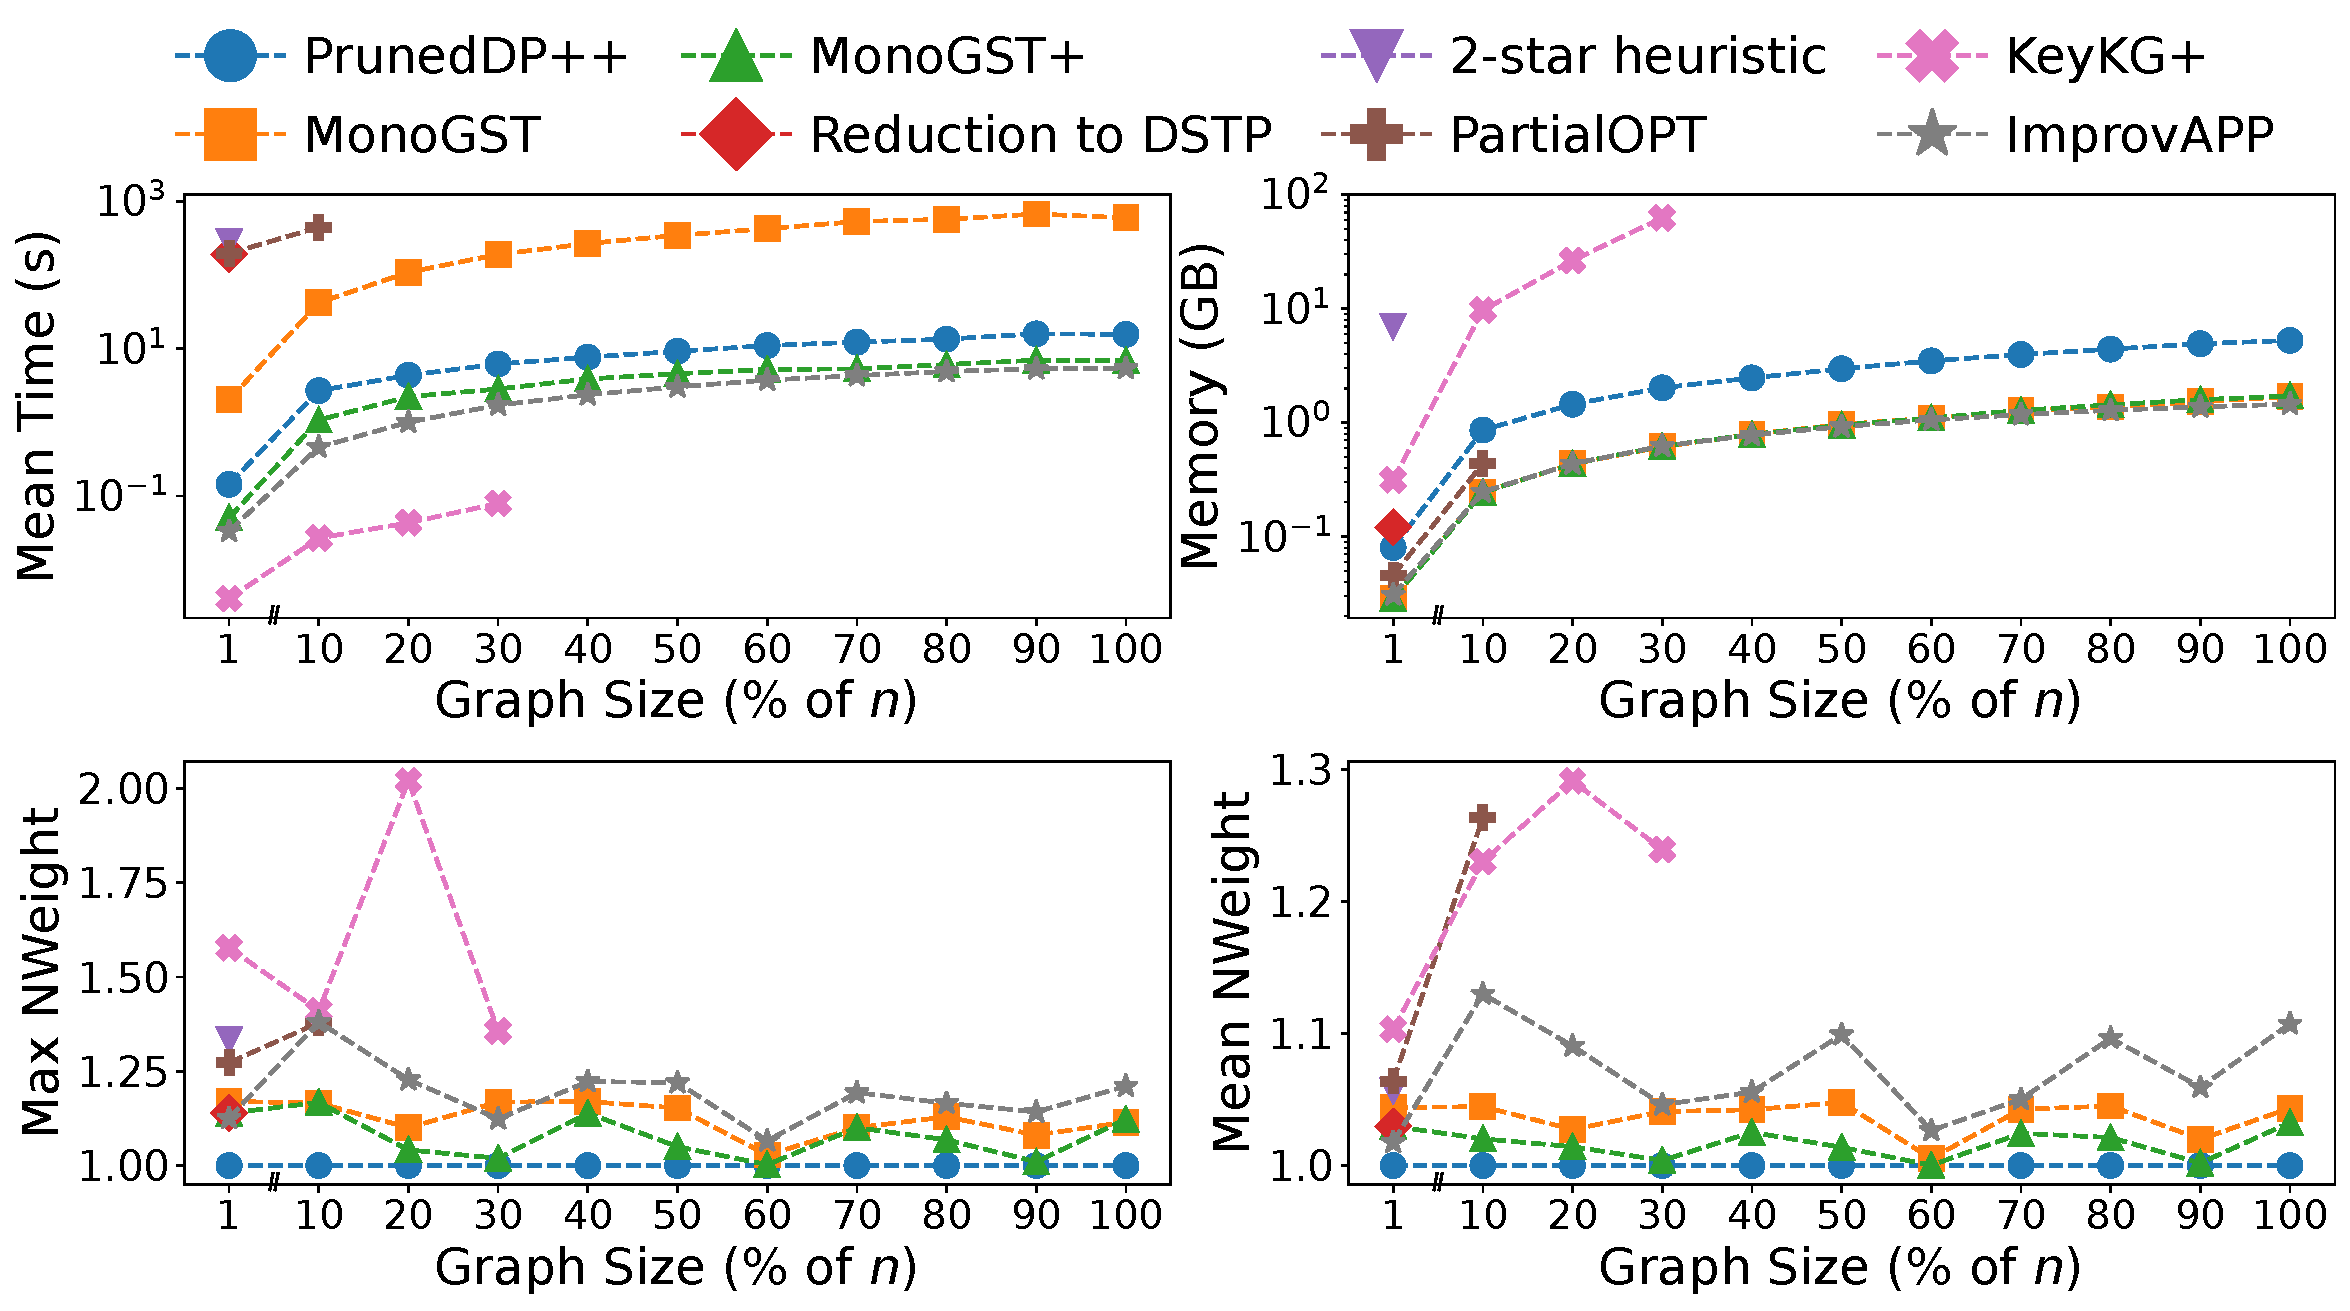
\includegraphics[width=\linewidth]{fig/subgraph/combined_metrics_2x2.pdf}
    \caption{Scalability analysis.}
    \label{fig: subgraph}
\end{figure}

\subsubsection{Experimental Results}

\dew{Figure~\ref{fig: subgraph} shows, for each algorithm on each graph, its mean running time, memory used, and maximum and mean NWeights over all GSTP instances.}

\dew{\textbf{Efficiency Results (Running Time and Memory Use).}
ImprovAPP and our \ImprovPTS are the fastest index-free algorithms and have the lowest memory use. Crucially, their time and space increase slowly with~$n$.
% The running time of \ImprovPTS increases smoothly from 0.05~seconds on the smallest subgraph to 6.82~seconds on the largest.
% The memory usage of \ImprovPTS increases from 0.029~GB to 1.716~GB.
Other algorithms that exhibit comparable scalability though slower include PrunedDP++ and our \Basic.}

\dew{The remaining algorithms show scalability limitations and their curves terminate early. The index building in KeyKG$^+$ uses a vast volume of memory and is complete within 24~hours only for the smallest four graphs. The reduction-to-DSTP approach, the 2‑star heuristic, and PartialOPT encounter timeouts on all GSTP instances on all but the smallest one or two graphs. The 2‑star heuristic also has the highest memory use, more than~7GB for the smallest graph.}

\dew{\textbf{Effectiveness Results (NWeight).}
For all approximation algorithms, their NWeights fluctuate when graph expands. On almost all graphs, our 2-star-based algorithms output better results than ImprovAPP and KeyKG$^+$ based on 1-star.
% ImprovPTS attains the lowest mean NWeight on 10 of the 11 subgraphs, and the lowest maximum NWeight on 7, with one additional tie. Its mean and maximum NWeights are always at most 1.033 and 1.167, respectively.
}

% Respond Reviewer #5 R5: In particular, the authors should clarify how timeout cases are handled in quality comparisons, and report whether the conclusions change under an evaluation that includes all instances (for example, by treating timeout cases conservatively). In addition, if polylogarithmic-approximation methods are too expensive for the full datasets, they should be evaluated on smaller graphs/subgraphs or otherwise discussed more explicitly to better position the proposed method.
\dew{\textbf{Concluding Remarks.}
Our \ImprovPTS is among the highest scalable algorithms and its finer solution quality remains consistent across different graph sizes, strengthening its practicality.}

% Respond Reviewer #4 R3: Although the authors vary the number of groups (g) and the average group size (f), Table 3 presents only aggregate results, failing to show how these parameters affect algorithm performance independently. The authors should include detailed sensitivity analyses, such as plots of runtime and NWeight against varying g and f, to demonstrate the algorithm's robustness across different query configurations.
\subsection{Robustness Analysis}
\label{subsec: sensitivity}

\dew{We analyzed how the number of groups~$g$ and the average group size~$f$ affect the performance of our \ImprovPTS.}

\subsubsection{Parameter Settings}

\dew{On DBLP, we followed the query generation scheme described in Section~\ref{sec:datasets} to generate more queries under extended parameter ranges: varying $g\in\{5,10,\dots,50\}$ with $f=200$, and varying $f\in\{200,400,\dots,2000\}$ with $g=5$.}
% again using 10 random queries per setting.

\begin{figure}[t]
    \centering
    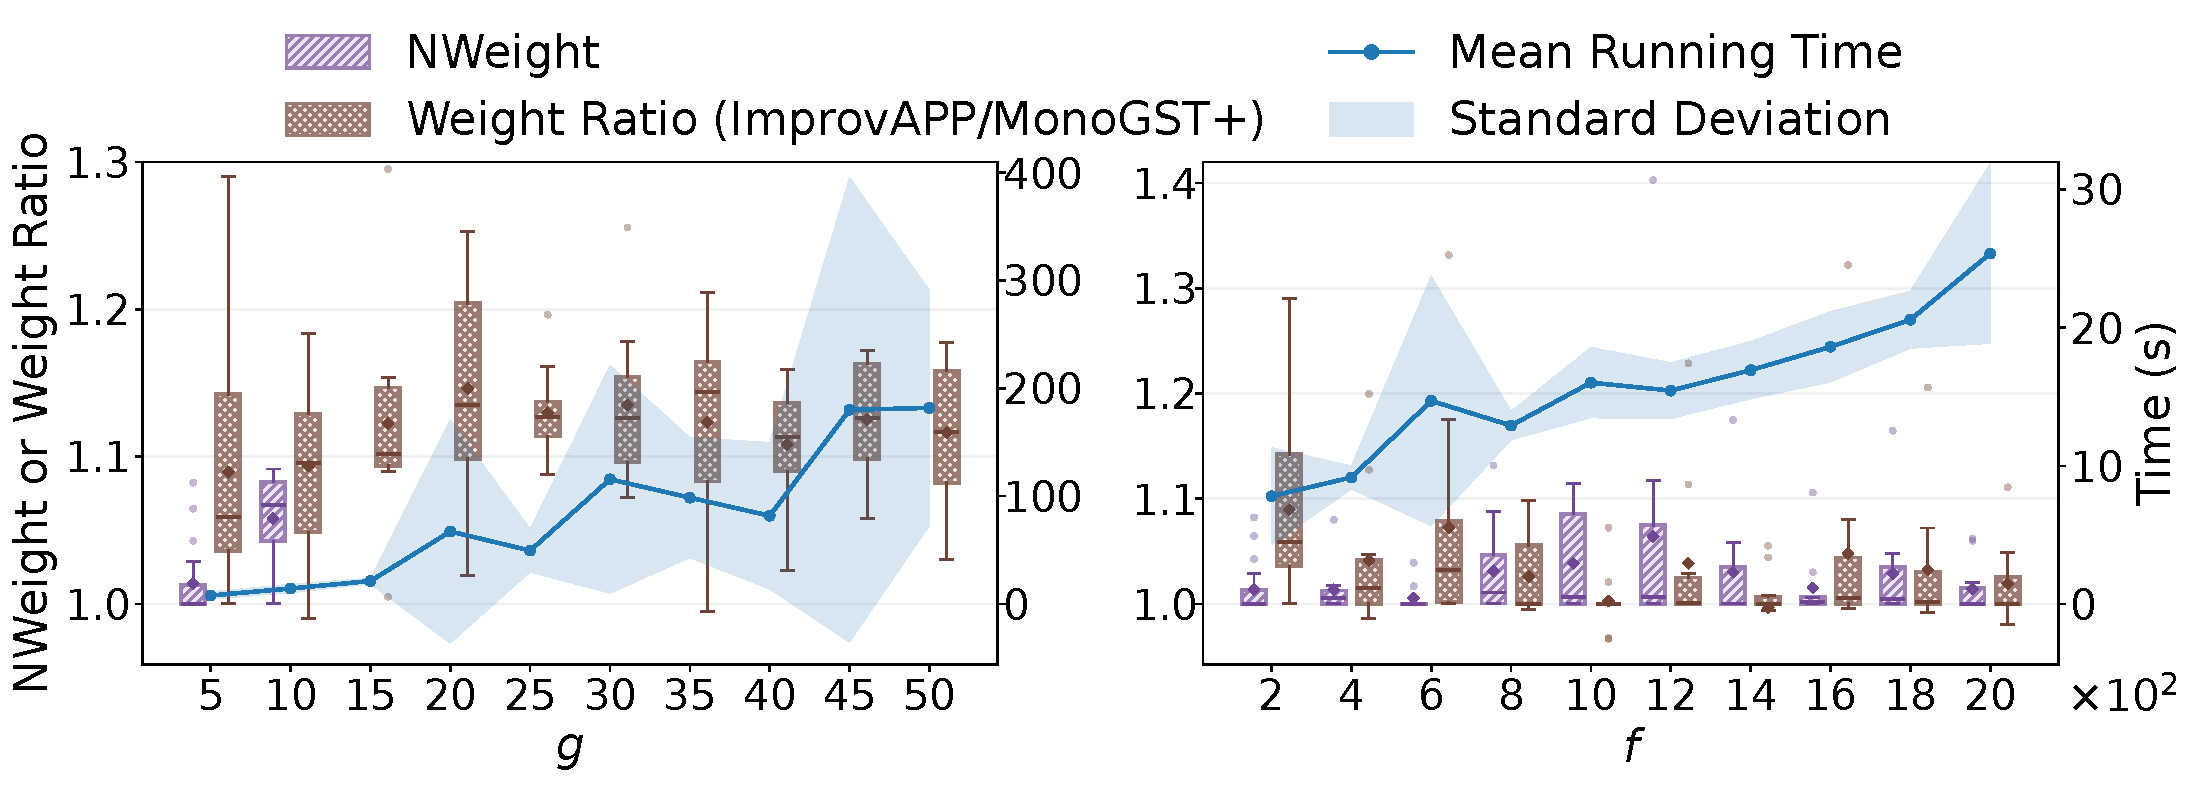
\includegraphics[width=\linewidth]{fig/big_g_f/DBLP_gfv_three_metrics_combined.pdf}
    \caption{Robustness analysis of \ImprovPTS.}
    \label{fig: sens_gf}
\end{figure}

\subsubsection{Experimental Results}

\dew{Figure~\ref{fig: sens_gf} plots the distributions of running time and NWeight of \ImprovPTS over all GSTP instances in each parameter setting. For $g>10$, the exact solver could not find a minimum-weight GST in reasonable time since its time complexity is exponential in~$g$, so NWeight became unavailable; compensating for that, we also calculated the ratio of the weight of the GST computed by our main baseline ImprovAPP to that by \ImprovPTS.}

% Respond Reviewer #2 R1: In the experiments, the values of g are set to [5, 8] which are too small. This setting is not super meaningful to me.
% To see this, according to Table 1, if g is such a small constant, the running time of ImprovAPP is bounded by O(m + n^2) which is better than the one of MonoGST+ O(nm + n^2). Moreover, in this case, the approximation ratios of both these algorithms are considered O(1).
% These assertions are also evidenced by the experimental results. In Table 3, the running time of ImprovAPP is faster than MonoGST+ in most of datasets (except for LinkedMDB) and its average NWeight is competitive to that of MonoGST+, where both of them are very close to 1.
% Therefore, from these experimental results, the effectiveness of MonoGST+ is less significant.

% Respond Reviewer #2 R3(?): As mentioned in O1, the practical performance of MonoGST+ seems not substantially better than the existing SOTA ImprovAPP.
% The authors need to design experiments to show the superiority of their algorithm.

% Respond Reviewer #5 R1: The revision should analyze how performance changes with the number of groups (g), ...
% Respond Reviewer #2 R2. The dedicated experimental study on impact of the average group sizes f is missing. It is unclear that why f is set to {200, 400, 800, 1600}.
% Experiments on f is needed. The impact of a large g with small f is unclear from the current experimental results.
\dew{\textbf{Efficiency Results (Running Time).}
In general, the mean running time increases near proportionally to~$g$ and~$f$, from~7.80 to 181.85~seconds when $g$~increases from~5 to~50, and from~7.80 to 25.37~seconds when $f$~increases from~200 to~2,000.}

\dew{\textbf{Effectiveness Results (NWeight).}
The mean NWeight fluctuates between~1.006 and~1.064 when $f$~changes from~200 to~2,000. It is also small when $g \leq 10$. For larger values of~$g$ such that NWeight is not calculable, the mean weight ratio of ImprovAPP to \ImprovPTS is kept between~1.108 and~1.146; it is also mostly above~1 when $f$~changes, showing that \ImprovPTS robustly delivers high-quality solutions and outperforms ImprovAPP.}
% The paired quality ratio is at least~1 on almost all settings and is within 0.4\% of parity in the only slightly unfavorable case.

\dew{\textbf{Concluding Remarks.}
The high accuracy of \ImprovPTS is insensitive to~$g$ and~$f$. Its running time is empirically linear in these parameters, conforming to our theoretical analysis in Section~\ref{sec:improve-time}.}

\begin{table}[t]
    \centering
    \caption{Ablation study of \ImprovPTS.}
    \label{table: abl}
    \small
    \begin{tabular}{l r @{\hspace{2pt}} l c r @{\hspace{2pt}} l}
    \toprule
    \multirow{2}{*}{Algorithm}
    & \multicolumn{2}{c}{\multirow{2}{*}{Mean Time (s) ${\scriptstyle\downarrow}$}}
    & \multicolumn{3}{c}{NWeight ${\scriptstyle\downarrow}$} \\
    \cline{4-6}
    & & & Max & \multicolumn{2}{c}{Mean}\\
    \midrule
%    \multicolumn{6}{c}{\emph{Experimental results on Toronto}} \\
     \ImprovPTS \emph{on Toronto} & 0.085 & \scriptsize{$\pm$ 0.041} & 1.417 & 1.026 & \scriptsize{$\pm$ 0.051} \\
     w/o suspension & 7.884 & \scriptsize{$\pm$ 5.873} & 1.417 & 1.025 & \scriptsize{$\pm$ 0.050}\\
     w/o suspension \& pruning & 11.819 & \scriptsize{$\pm$ 9.734} & 1.417 & 1.025 & \scriptsize{$\pm$ 0.049} \\
     w/o re-selection & 0.088 & \scriptsize{$\pm$ 0.043} & 1.417 & 1.056 & \scriptsize{$\pm$ 0.069} \\
    \dew{median group} & 0.101 & \scriptsize{$\pm$ 0.041} & 1.417 & 1.026 & \scriptsize{$\pm$ 0.051} \\
    \dew{largest group} & 0.101 & \scriptsize{$\pm$ 0.041} & 1.417 & 1.026 & \scriptsize{$\pm$ 0.051} \\
    % \ImprovPTS \scriptsize{(medium-group)} & 0 & 0.101 & \scriptsize{$\pm$ 0.041} & 1.417 & 1.026 & \scriptsize{$\pm$ 0.051} \\
    % \ImprovPTS \scriptsize{(max-group)} & 0 & 0.101 & \scriptsize{$\pm$ 0.041} & 1.417 & 1.026 & \scriptsize{$\pm$ 0.051} \\
    \hline
%    \multicolumn{6}{c}{\emph{Experimental results on MovieLens}} \\
     \ImprovPTS \emph{on MovieLens} & 1.599 & \scriptsize{$\pm$ 0.316} & 1.192 & 1.015 & \scriptsize{$\pm$ 0.035}\\
     w/o suspension & 49.986 & \scriptsize{$\pm$ 35.506} & 1.192 & 1.015 & \scriptsize{$\pm$ 0.035} \\
     w/o suspension \& pruning & 51.145 & \scriptsize{$\pm$ 36.323} & 1.192 & 1.015 & \scriptsize{$\pm$ 0.035} \\
     w/o re-selection & 1.649 & \scriptsize{$\pm$ 0.274} & 1.192 & 1.025 & \scriptsize{$\pm$ 0.042} \\
    \dew{median group} & 1.653 & \scriptsize{$\pm$ 0.303} & 1.192 & 1.015 & \scriptsize{$\pm$ 0.035} \\
    \dew{largest group} & 1.600 & \scriptsize{$\pm$ 0.269} & 1.192 & 1.015 & \scriptsize{$\pm$ 0.035} \\
    \hline
%    \multicolumn{6}{c}{\emph{Experimental results on DBLP}} \\
     \ImprovPTS \emph{on DBLP} & 15.876 & \scriptsize{$\pm$ 8.242} & 1.209 & 1.032 & \scriptsize{$\pm$ 0.042}\\
     w/o suspension & 1700.880 & \scriptsize{$\pm$ 1247.202} & 1.209 & 1.031 & \scriptsize{$\pm$ 0.041}\\
     w/o suspension \& pruning & 2394.501 & \scriptsize{$\pm$ 1834.009} & 1.209 & 1.031 & \scriptsize{$\pm$ 0.041} \\
     w/o re-selection & 16.669 & \scriptsize{$\pm$ 10.110} & 1.241 & 1.058 & \scriptsize{$\pm$ 0.053}\\
    \dew{median group} & 16.261 & \scriptsize{$\pm$ 8.354} & 1.209 & 1.032 & \scriptsize{$\pm$ 0.042} \\
    \dew{largest group} & 16.275 & \scriptsize{$\pm$ 8.524} & 1.209 & 1.032 & \scriptsize{$\pm$ 0.042} \\
    \midrule
%    \multicolumn{6}{c}{\emph{Experimental results on LinkedMDB}} \\
     \ImprovPTS \emph{on LinkedMDB} & 0.756 & \scriptsize{$\pm$ 0.671} & 1.223 & 1.040 & \scriptsize{$\pm$ 0.057} \\
     w/o suspension & 1.544 & \scriptsize{$\pm$ 1.684} & 1.223 & 1.038 & \scriptsize{$\pm$ 0.055}\\
     w/o suspension \& pruning & 1.572 & \scriptsize{$\pm$ 1.732} & 1.223 & 1.038 & \scriptsize{$\pm$ 0.055}\\
     w/o re-selection & 0.753 & \scriptsize{$\pm$ 0.667} & 1.261 & 1.053 & \scriptsize{$\pm$ 0.068}\\
    \dew{median group} & 0.763 & \scriptsize{$\pm$ 0.678} & 1.246 & 1.034 & \scriptsize{$\pm$ 0.055} \\
    \dew{largest group} & 0.761 & \scriptsize{$\pm$ 0.677} & 1.246 & 1.034 & \scriptsize{$\pm$ 0.055} \\
    \hline
%    \multicolumn{6}{c}{\emph{Experimental results on DBpedia}} \\
     \ImprovPTS \emph{on DBpedia} & 7.717 & \scriptsize{$\pm$ 3.538} & 1.204 & 1.012 & \scriptsize{$\pm$ 0.029}\\
     w/o suspension & 39.992 & \scriptsize{$\pm$ 107.420} & 1.204 & 1.012 & \scriptsize{$\pm$ 0.029}\\
     w/o suspension \& pruning & 41.697 & \scriptsize{$\pm$ 110.882} & 1.204 & 1.012 & \scriptsize{$\pm$ 0.028}\\
     w/o re-selection & 7.560 & \scriptsize{$\pm$ 3.447} & 1.204 & 1.016 & \scriptsize{$\pm$ 0.032}\\
    \dew{median group} & 7.853 & \scriptsize{$\pm$ 3.566} & 1.204 & 1.012 & \scriptsize{$\pm$ 0.029} \\
    \dew{largest group} & 7.797 & \scriptsize{$\pm$ 3.560} & 1.204 & 1.012 & \scriptsize{$\pm$ 0.029} \\
    \bottomrule
    \end{tabular}
\end{table}

\subsection{Ablation Study}
\label{subsec: able}

\subsubsection{Variant Settings}

We conducted an ablation study by implementing and comparing five variants of \ImprovPTS, aiming to isolate and quantify the effects of its key components.

The variant \textbf{w/o suspension} replaces our suspendable Dijkstra's algorithm (Section~\ref{subsec: sec_dub}) with the standard Dijkstra's algorithm to compute SSSP from each root $r \in K_1$ in a manner identical to that in \Basic (line~10).
The variant \textbf{w/o suspension \& pruning} further disables our prefix pruning (Section~\ref{subsec: mono_upt}) and enumerates each prefix~$p$ from~2 to~$g$ in a manner identical to that in \Basic (line~14).
The variant \textbf{w/o re-selection} replaces our path re-selection (Section~\ref{subsec: sec_rebuild}) with the naive method for converting a 2-star into a GST described in Section~\ref{subsec: 2-star} in a manner identical to that in \Basic (lines~19--21).
Note that suspension and prefix pruning mainly optimize running time, while path re-selection focuses on solution quality, addressing different aspects of performance.

\dew{\Improved enumerates the vertices in the smallest group as the root of a 2-star (line~1). Differently, the variants \textbf{median group} and \textbf{largest group} choose a group of median size and the largest group as~$K_1$ to enumerate, respectively.}

\subsubsection{Experimental Results}
\label{subsubsec: abl_result}
Table~\ref{table: abl} shows, for each variant on each dataset, its mean running time, and maximum and mean NWeights over all GSTP instances. For precisely reflecting performance difference, we removed per-run time limit from this ablation study.

% Respond Reviewer #5 R1: The revision should..., quantify the benefit of early termination in suspendable Dijkstra (e.g., visited nodes/work saved versus full SSSP), and evaluate the effect of prefix pruning. (最后半句在 Detailed Evaluation 里面说 The effectiveness of prefix pruning is not evaluated as a function of g. 还没加）
\textbf{Efficiency Results (Running Time).}
The suspendability mechanism is the key driver behind the efficiency of \ImprovPTS. It enables speedups of 1--2 orders of magnitude on Toronto, MovieLens, and DBLP, and $2\times$--$5\times$ on LinkedMDB and DBpedia. \dew{With suspendability on different datasets, only an average of 0.02\%--20\% of all vertices are visited when Dijkstra's algorithm is terminated.}

Prefix pruning provides both theoretical and empirical benefits: it reduces the time complexity by a factor of~$g$, and produces consistent speedups across all datasets, up to 29\%--33\% on Toronto and DBLP.
% 总体而言，g 越大增量越多（括号里面举个例子，当 g 从多少到多少 在某个数据集上）
\dew{The benefit becomes more pronounced as $g$~increases, e.g.,~from~21\% to~42\% as $g$~increases from~5 to~8 on Toronto.}

\dew{Switching from the smallest group to the median or largest group leads to consistent increases in running time, up to~19\% on Toronto.}

\textbf{Effectiveness Results (NWeight).}
Path re-selection yields consistent, though modest, quality improvements on all datasets, up to 2\%--3\% reduction in mean NWeight on Toronto and DBLP. Incurring negligible time cost, it represents a net-positive trade-off between effectiveness and efficiency.

\dew{Enumerating the smallest, median, or largest group has little effect on solution quality on most datasets.}

% 使用 suspensio 后实际访问的节点的平均比例
% DBLP:      0.0009301625
% DBpedia:   0.0585949977
% LinkedMDB: 0.1961901100
% MovieLens: 0.0002347000
% Toronto:   0.0007252625

% (w/o suspension & pruning - w/o suspension) / w/o suspension & pruning 不同 g 的 结果
% DBLP
%   g=5: 0.1873611037
%   g=6: 0.2412399713
%   g=7: 0.3068331645
%   g=8: 0.3628756823
% DBpedia
%   g=1: -0.3333333333  skipped_zero=1
%   g=2: -0.0090308388
%   g=3: -0.0001541120
%   g=4: 0.0155753004
%   g=5: 0.0201601114
%   g=6: 0.0313407780
%   g=7: 0.0701080392
%   g=8: 0.0895480933
%   g=9: 0.1030067716
%   g=10: 0.1083023208
% LinkedMDB
%   g=1: -0.0968253968  skipped_zero=5
%   g=2: -0.0376935060
%   g=3: -0.0279413468
%   g=4: 0.0386849984
%   g=5: -0.0015366147
%   g=6: -0.0675875087
%   g=7: -0.0019840130
%   g=8: 0.0341245371
%   g=9: 0.0717124332
%   g=10: 0.0146946877
% MovieLens
%   g=5: 0.0208141968
%   g=6: 0.0188620342
%   g=7: 0.0268043835
%   g=8: 0.0319513820
% Toronto
%   g=5: 0.2139474811
%   g=6: 0.3015960823
%   g=7: 0.3539243170
%   g=8: 0.4153350093

\textbf{Concluding Remarks.}
In summary, all three optimizations integrated into \ImprovPTS collectively establish its superiority over \Basic in terms of efficiency and effectiveness. These novel techniques enable \ImprovPTS to achieve state-of-the-art performance among approximate GST algorithms. \dew{It is also cost-effective to enumerate the vertices in the smallest group as the root of a 2-star.}
\section{Related Work}
\label{sec: relatedwork}

% Table~\ref{table: Algorithms Comparison} summarizes the time complexities and approximation ratios of representative GST algorithms.

\subsection{Sublinear-Approximation Algorithms}
\label{subsec: sub-alg}
% Our algorithms belong to this category.

The 2-star concept is first introduced in~\cite{dstar1} to solve GSTP, where a heuristic two-step algorithm achieves an $O(\sqrt{g}\ln g)$ approximation, and is later generalized to $d$-star~\cite{dstar2}.
\emph{Our holistic analysis improves this ratio to $O(\sqrt{g})$.}
Besides, the algorithms in \cite{dstar1,dstar2} incur the high cost of computing all-pairs shortest paths.
\emph{Our suspendable Dijkstra’s algorithm calculates distances lazily and supports early termination.}
Although both~\cite{dstar1} and our approach employ greedy set cover, \emph{we define a novel greedy function whose monotonicity and unimodality enable efficient pruning.}
This combination of pay-as-you-go distance calculation and a pruning-friendly greedy function makes our \ImprovPTS a practical solution for large GSTP instances.
% its running time is $O(\tau + (ng)^d)$, where $\tau$ is an upper bound on computing all-pairs shortest paths

GSTP can be reduced to DSTP~\cite{D_STP} where the $d$-star-based algorithm achieves an $O(\sqrt{g})$ approximation in $O(n^d g^{2d})$ time, not efficient on large graphs even for $d=2$.
Using a more scalable DST algorithm~\cite{DiST} can reduce the time complexity of solving DSTP to $O(mg+ng\log n)$. Nevertheless, the approach still requires processing up to $n$~DSTP instances, each involving $g$~SSSP computations, amounting to a total of $gn$~computations.
By contrast, \emph{our algorithms perform at most $(g+n)$~SSSP computations,} accounting for their orders-of-magnitude speedup in our experiments.

% The polylog-approximation algorithms in~\cite{PolyAppr_1, PolyAppr_2} use tree metrics with stretch $O(\log n)$ to reduce the problem to GSTP on trees. For GSTP on a tree,~\cite{PolyAppr_1} applies a separation oracle to solve a linear program with an exponential number of constraints, or alternatively leverages the max-flow min-cut theorem to reinterpret the constraints so that they can be handled in polynomial time. In contrast,~\cite{PolyAppr_2} first performs a height-reducing transformation and a degree-reducing transformation to obtain a tree of height $O(\log n/\log\log n)$ and maximum degree $O(\log n)$; it then applies a greedy strategy, further reducing the number of recursive calls via geometric search and by pruning subtrees that cover few groups, together with additional preprocessing, to achieve a theoretical polynomial-time bound.

% Respond Reviewer #5 R5: In particular, the authors should clarify how timeout cases are handled in quality comparisons, and report whether the conclusions change under an evaluation that includes all instances (for example, by treating timeout cases conservatively). In addition, if polylogarithmic-approximation methods are too expensive for the full datasets, they should be evaluated on smaller graphs/subgraphs or otherwise discussed more explicitly to better position the proposed method.
Polylogarithmic-approximation algorithms~\cite{PolyAppr_1, PolyAppr_2} relax GSTP to its variant on a tree with stretch $O(\log n)$, and invoke heavy subroutines such as solving linear programs with exponentially many constraints. \dew{As noted in their papers, they incur large hidden constants and accumulated polylogarithmic factors, hard to perform efficiently in practice.}
GSTP can also be reduced to the Steiner Tree Problem (STP)~\cite{ST_noappr}, but an approximation ratio is guaranteed only if using an exact, exponential-time STP solver.
\emph{Consequently, the algorithms discussed above are more oriented towards theoretical analysis than practical deployment,} thus omitted from our experiments.

\subsection{Linear-Approximation Algorithms}
\label{subsec: line-alg}
% Existing algorithms that scale to large graphs are typically $O(g)$-approximation algorithms; exact methods can be applied to large instances only with difficulty, suffer occasional timeouts, are on average slower by several orders of magnitude, and generally require $g$ to be small.

% This class of algorithms is usually more practical for large graphs but offers weaker guarantees on solution quality.

KeyKG$^+$~\cite{KeyKG} as an extension of 1-star achieves a $(g-1)$~approximation. To accelerate the search for the closest uncovered group to merge into the current GST, it uses a distance index~\cite{PLL}.
% to handle vertex-to-group distance queries.
Building this index is computationally expensive and may not scale to very large graphs, such as the DBLP dataset in our experiments.
% identifies a core-vertex set to find a tightly clustered set of vertices and a corresponding root, and then greedily connects the group closest to the current tree.

Among index-free methods that guarantee a $(g-1)$~approximation, ImprovAPP~\cite{ImprovAPP} performs SSSP computations and uses a priority queue to track the uncovered group closest to each vertex in the current GST. PartialOPT~\cite{ImprovAPP} improves the approximation to~$(g-h+1)$ by introducing a parameter $h \in [2,g]$ and invoking an exact GST solver~\cite{KS_5} on $h$~groups. Its time complexity grows exponentially with~$h$; in practice, a small~$h$ (e.g.,~$h=3$) must be used, resulting in marginal quality gains.
% Moreover, because the coupling between the exact and approximate components is rather intricate, they often fail to realize the strengths of either side in terms of both running time and solution quality in practice

Earlier methods also achieve an $O(g)$-approximation, such as BANKS~\cite{BANKS}, its improved variant BANKS-II~\cite{BANKS2} \dew{that} employs bidirectional search, and BLINKS~\cite{BLINKS} \dew{that} partitions the graph into blocks and builds a block-level index for search pruning.
% BANKS performs reverse searches from each group and iteratively merges paths to form a GST

The algorithms discussed above are predominantly 1-star-based, which trades off a linear approximation ratio in~$g$ for efficiency. By contrast, building on the 2-star framework, \emph{our \ImprovPTS guarantees a strictly better approximation ratio while maintaining its running time comparable to the state-of-the-art index-free linear-approximation algorithms.} Therefore, our work bridges a long-standing gap that has traditionally forced a choice between high-quality approximation and scalable, efficient computation.

\subsection{Exact Algorithms} 

Prominent exact GST solvers include DPBF~\cite{KS_5}, which employs best-first dynamic programming, and its successor PrunedDP++~\cite{PrunedDP} based on A* search. Both of them exhibit exponential time complexity and limited scalability. \emph{This body of work is largely orthogonal to ours, as they pursue different aims and adopt disparate methodologies.} In our experimental setup, PrunedDP++ serves a specific role: it provides the optimum GST weights needed to compute NWeight for quantifying the empirical approximation ratios of our algorithms.
% DPBF is a dynamic program whose state encodes the current subtree root together with the set of already covered groups; transitions merge two subtrees sharing the same root and expand the current subtree from the root. PrunedDP++ leverages A* search to prune DPBF's state space and generates the solution progressively, yielding substantial speedups.
% \emph{In contrast to the $d$-star paradigm adopted by approximation algorithms, exact methods must perform dynamic programming over coverings of arbitrary subsets of terminal groups, which makes them infeasible even when the number of groups is moderately large and thus substantially limits their applicability in practice.}

% For sublinear-approximation algorithms, the rooted steiner 2-star heuristic algorithm in ~\cite{dstar1} introduced $2$-star, approximated via a set cover algorithm similar to ours, and proved a $(1+\ln \tfrac{g}{2})\sqrt{g}$ approximation ratio; however, it requires all-pairs shortest paths, which is impractical. \cite{dstar2} extend $2$-star to $d$-star without altering the algorithmic techniques; its running time is $O(\tau + (ng)^d)$, where $\tau$ is an upper bound on computing all-pairs shortest paths. 

% The Directed Steiner Tree variant proposed in ~\cite{D_STP} also employs $d$-star and can be reduced to GSTP. For $d=2$, it achieves a $\sqrt{g}$ approximation ratio; however, its theoretical $O(n^d g^{2d})$ time complexity is high, rendering it difficult to run in practice. By contrast, DiST in~\cite{DiST} achieves a faster running time of $O(mg+ng\log n)$ while maintaining an $O(\sqrt g)$ approximation ratio. Note that reducing DSTP to GSTP requires enumerating the root vertex; consequently, such reduction-based approaches must solve $O(n)$ DSTP instances to obtain a solution for GSTP.

% The polylog-approximation algorithms in~\cite{PolyAppr_1, PolyAppr_2} use tree metrics with stretch $O(\log n)$ to reduce the problem to GSTP on trees. For GSTP on a tree,~\cite{PolyAppr_1} applies a separation oracle to solve a linear program with an exponential number of constraints, or alternatively leverages the max-flow min-cut theorem to reinterpret the constraints so that they can be handled in polynomial time. In contrast,~\cite{PolyAppr_2} first performs a height-reducing transformation and a degree-reducing transformation to obtain a tree of height $O(\log n/\log\log n)$ and maximum degree $O(\log n)$; it then applies a greedy strategy, further reducing the number of recursive calls via geometric search and by pruning subtrees that cover few groups, together with additional preprocessing, to achieve a theoretical polynomial-time bound. Overall, these algorithms are geared more toward theoretical guarantees than practical performance, and are therefore inefficient in practice. GSTP can also be reduced to the Steiner Tree Problem (STP)~\cite{ST_noappr}, but this requires exact STP solvers; otherwise, the result can be arbitrarily bad.

\section{Conclusion}
\label{sec: conclusion}

Our work reconciles the long-standing trade-off between sublinear approximation and practical running time for GSTP through: (i)~\BasicPTS, which, via a holistic analysis of its two-step greedy approximation, achieves an $O(\sqrt{g})$~ratio; and (ii)~\ImprovPTS, which further incorporates a suspendable search mechanism and a pruning strategy that exploits the monotonicity and unimodality of the greedy function to match the efficiency of state-of-the-art linear-approximation solvers. This combined effectiveness and efficiency is validated by an extensive evaluation across five real-world datasets spanning tasks such as property search in road networks, team formation in social networks, and keyword-based exploration of KGs, where \ImprovPTS produces the highest-quality GSTs among approximation algorithms without compromising on speed.

While these results are promising, several important limitations point to clear avenues for advancement. First, regarding efficiency, our method is on par with the fastest existing index-free baselines but has not advanced beyond; its reliance on $g$~full SSSP computations remains a notable limitation at scale. Second, concerning approximation quality, our work is currently limited to the $d=2$ case of the $d$-star framework, despite the fact that larger~$d$ generally yields higher quality. Future directions, therefore, involve: (i)~developing lightweight, updatable indices (rather than the heavy, static one in KeyKG$^+$) to accelerate distance queries; and (ii)~deeply exploring the $d$-star structure to efficiently expand the search space.
% (ii)~tightening the theoretical analysis to reduce computational costs without compromising solution quality;

% Despite these encouraging results, there remains room for improvement. In particular, our practical running time does not yet surpass the speed bottleneck of the fastest index-free algorithms, and our algorithm still performs \(g\) full shortest-path computations, which may become costly when the number of groups is large~\cite{KGS_1}. A promising direction is to accelerate distance evaluation by introducing lightweight, fast-to-build, and dynamically maintainable indices, or by developing a tighter theoretical  characterization that further reduces the number of shortest-path computations without sacrificing solution quality.

\begin{acks}
This work was supported by the Noncommunicable Chronic Diseases-National Science and Technology Major Project (2025ZD0544900), the Fundamental Research Funds for the Central Universities (No. 2026300429), the Fundamental and Interdisciplinary Disciplines Breakthrough Plan of the Ministry of Education of China (No. JYB2025XDXM118), and the ``111 Center'' (No. B26023).
\end{acks}

\clearpage

\bibliographystyle{ACM-Reference-Format}
\balance
\bibliography{main}

\end{document}
\endinput